	\chapter{Ο πυρήνας της Μηχανής}
	
	Μια βιβλιοθήκη (framework) η οποίο επεκτείνεται και διακλαδώνεται σε πολλές υποβιβλιοθήκες, στηρίζεται στη θεμελιώση ενός πηρύνα (framework core) ώστε να μπορέσει να επεκταθεί με σταθερότητα και συνέχεια. Το \gls{API} του πυρήνα πρέπει να είναι εύκολο στην κατανόηση, να αποτελείται από αυτοεπεξηγούμενες αφαιρέσεις, οι οποίες εκθέτουν μόνο τα απολύτως απαραίτητα, ώστε οι υποβιβλιοθήκες που χρησιμοποιούν τον πυρήνα να μην δεσμεύονται σε υλοποιήσεις, να περιορίζει τον χρήστη σε συγκεκριμένα στάδια χρήσης για αποφυγή απρόβλεπτων συμπεριφορών και να προσφέρει δυνατότητες επεκτασιμότητας.  \cite{jaroslav08} Ο πυρήνας περιέχει υποσυστήματα τα οποία μπορούν να χρησιμοποιηθούν τη δημιουργία διαφόρων ειδών παιχνιδιών.
		
	\section{Κύκλος ζωής πυρήνα}	
	Κάθε οντότητα από τη στιγμή της δημιουργίας της στο περιβάλλον της μηχανής μέχρι την καταστροφής της και διαγραφή της από τη μνήμη, περνά από κάποια προκαθορισμένα στάδια τα οποία εκτελούνται ανάλογα με την κατάσταση του υλικού και του λογισμικού. Τα στάδια αυτά περιγράφονται στο διάγραμμα \ref{fig:corelifecycle} και είναι τα παρακάτω:
	
	\begin{description}
		\item [Initialization] To initialization (προετοιμασία) εκτελείται μια φορά κατά τη δημιουργία του παιχνιδιού.
		\item [Game loop] Το game loop (βρόγχος παιχνιδιού) εκτελείται με σταθερό χρονικο βήμα σε βρόγχο.
		\item [Disposing] To disposing εκτελείται μια φορά στην έξοδο. 
	\end{description}
	
	\begin{figure}[h!]
		\centering
		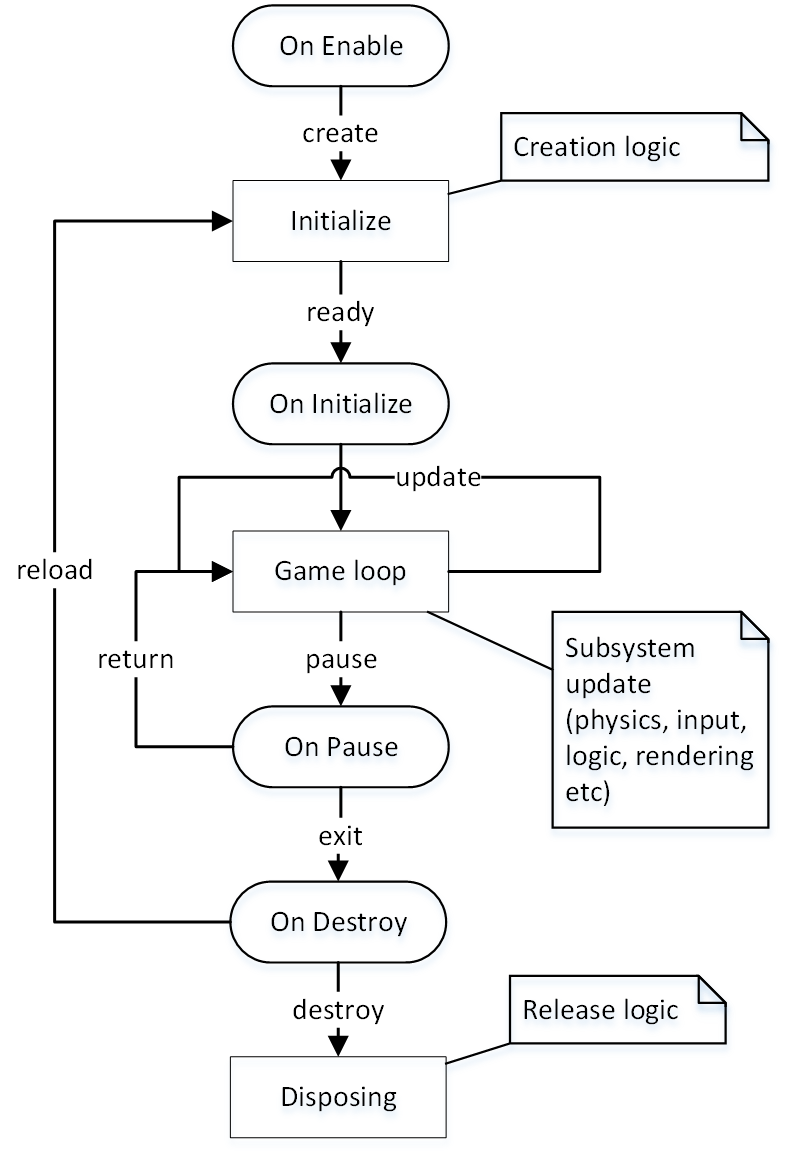
\includegraphics[width=80mm]{Images/core_lifecycle}
		\caption{Κύκλος ζωής του πυρήνα}
		\label{fig:corelifecycle}
	\end{figure}
		
	\subsection{Βρόγχος παιχνιδιού}
	Ο βρόγχος του παιχνιδιού (game loop) εγκυάται τη συνεπής ενημέρωση των υποσυστημάτων ανάλογα με το προκαθορισμένο χρονικό βήμα. Χωρίς το ανεξάρτητο σύστημα ενημέρωσης υποσυστημάτων, η ενημέρωση θα γινόταν στον κύκλο εκτέλεσης του επεξεργαστή με αποτέλεσμα την διαφορετική εμπειρία ανά επεξεργαστή και μηχάνημα. Όπως παρουσιάζεται στο σχήμα \ref{fig:gameloops}, όλα τα υποσυστήματα του παιχνιδιού ενημερώνονται στον βρόγχο του παιχνιδιού  .
	
	Το κάθε υποσύστημα έχει διαφορετικές απαιτήσεις για τη βέλτιστη και επιθυμητή λειτουργία. Το σύστημα συγκρούσεων χρειάζεται να ενημερώνεται εκατό φορές το δευτερόλεπτο, ενώ το σύστημα τεχνητής νοημοσύνης δύο φορές το δευτερόλεπτο \cite{gregory2009game}. Η πιο συνηθισμένη τεχνική είναι να υπάρχουν δύο κύριοι βρόγχοι ενημέρωσης (update loops):
	\begin{description}
	\item [Βρόγχος παιχνιδιού] Στο βρόγχο παιχνιδιού ενημερώνονται όλα τα υποσυστήματα όπως το υποσύστημα φυσικής, λογικής, δυναμικών κλπ.
	\item [Rendering loop] Στο rendering loop (βρόχο απόδοσης) οποίο γίνονται οι κλήσεις στην κάρτα γραφικών και ενημερώνεται στις 50-60 φορές το δευτερόλεπτο με αποτέλεσμα η οθόνη να ενημερώνεται στα 50-60 \gls{FPS}.
	\end{description}
	
	Η διαφορά του χρόνου μεταξύ των ενημερώσεων πρέπει να είναι εγγυημένη. Για παράδειγμα σε μια μηχανή στην οποία το rendering loop τρέχει στα 60 \gls{FPS} υπάρχει η συχνότητα ενημέρωσης:
	\begin{equation}
	 F = 1/T =>  F = 1000ms/60 => F = 16ms. 
	\end{equation}
	Για να μπορεί να εγγυάται το σύστημα αυτή την αναλογία, πρέπει η μηχανή να μετράει και να αποθηκεύει στη μνήμη τη διαφορά χρόνου μεταξύ κάθε κλήσης, να εκτελεί τον κώδικα στο συγκεκριμένο βρόχο και για τον υπόλοιπο χρόνο το νήμα (thread) στο οποίο εκτελείται η λογική ενημέρωσης του παιχνιδιού να κοιμάται (sleep).
	
	\begin{figure}[h!]
		\centering
		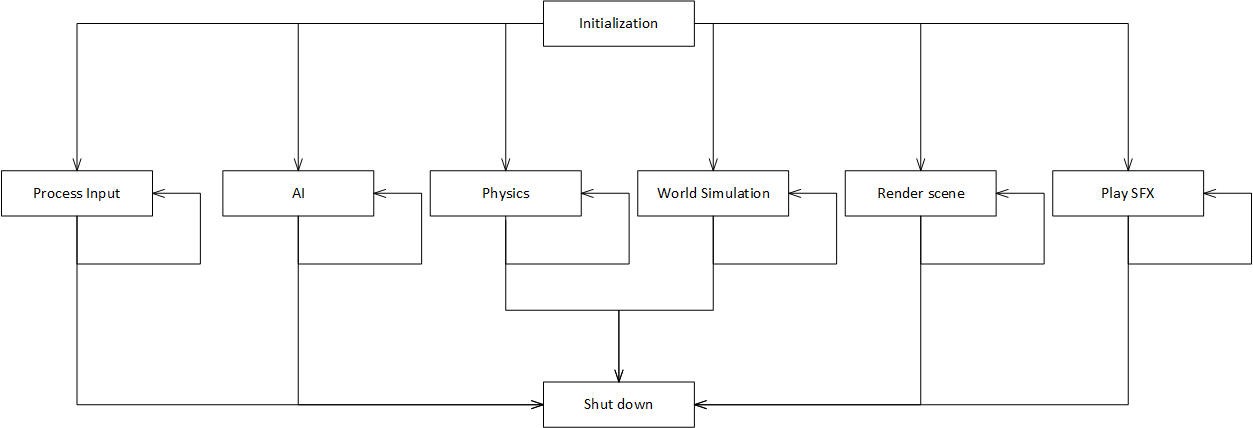
\includegraphics[width=160mm]{Images/gameloops_update}
		\caption{Βρόγχος παιχνιδιού}
		\label{fig:gameloops}
	\end{figure}
		
	\paragraph{Χρόνος}
	Η έννοια της διάρκειας και του χρόνου στα συστήματα πραγματικού χρόνου πρέπει να αντιμετωπίζεται απομονωμένα. Ο χρόνος του παιχνιδιού  είναι ανεξάρτητος από τον πραγματικό χρόνο. Η ενημέρωση και η λογική των συστημάτων γίνεται με βάση τη διαφορά χρόνου μεταξύ ενημερώσεων. Με αυτή την στρατηγική, η εμπειρία δεν διαφοροποιείται με λιγότερα \gls{FPS} και ένα animation το οποίο αποδίδεται σε πραγματικό χρόνο, μπορεί να αποδοθεί αντίστροφα ή με διπλάσια ταχύτητα, αν το χρονοδιάγραμμα στο οποίο ανταποκρίνεται, χειρίζεται τον χρόνο διαφορετικά.
	Όλα τα συστήματα ενημερώνονται γραμμικά συναρτήσει μιας αφαίρεσης η οποία αντιπροσωπεύει τη διαφορά χρόνου.
	\subsection{Υποσυστήματα}
	Το κάθε υποσύστημα δημιουργείται, ενημερώνεται και καταστρέφεται μέσα στο γενικό κύκλο ζωής του πηρύνα. Το κάθε υποσύστημα έχει εσωτερικά το δικό του κύκλο ζωής και κύκλο ενημέρωσης ο οποίος λειτουργεί μέσα στην έκταση του εξωτερικού κύκλου ζωής.
	
	\subsection{Τεχνικές Ενημέρωσης Υποσυστημάτων}
	Τα υποσυστήματα αν και απομονωμένα και χωρίς αλληλεξαρτήσεις πρέπει με κάποιο τρόπο να ενημερώνονται και να επικοινωνούν μεταξύ τους ή να στέλνουν μηνύματα όταν συμβεί κάποιο γεγονός. Οι τεχνικές ενημέρωσης υποσυστημάτων είναι οι παρακάτω:
	\begin{description}
	\item [Message Pumps] Τα υποσυστήματα στέλνουν μηνύματα σε ένα message bus και τα συστήματα ενημερώνονται όταν εξυπηρετείται το μήνυμα. Παραμένουν άεργα εφόσον δεν υπάρχει μήνυμα προς εξυπηρέτηση \cite{Erl:2009:SDP:1538586}.
	\item [Call-back driven] Tα υποσυστήματα παρέχουν call-back λειτουργικότητα, δηλαδή τη δυνατότητα δήλωσης κώδικας ο οποίος θα εκτελεστεί κατά κάποιο συμβάν. Ένα συμβάν μπορεί να είναι η σύγκρουση μεταξύ δύο αντικειμένων ή η είσοδος κάποιου παίχτη στον κόσμο. Ο χρήστης μπορεί για παράδειγμα να δηλώσει ότι όταν συμβεί σύγκρουση μεταξύ του παίχτη και του εχθρού, ο παίχτης θα χάσει ζωή.
	\end{description}
		
	\section{Διαχείριση οθονών}
	Σε ένα τυπικό χρόνο εκτέλεσης ενός παιχνιδιού, το παιχνίδι περνά από διάφορες καταστάσεις. Οι καταστάσεις αυτές μπορεί να είναι η προσωρινή παύση, ένα μενού ρυθμίσεων ένα \gls{GUI} επιλογών το οποίο επικαλύπτει το τρέχον παιχνίδι ή αποδίδεται στον ίδιο render buffer. Το παιχνίδι χωρίζεται σε σκηνές, σε επίπεδα και σε χάρτες οι οποίες έχουν ξεχωριστό τρόπο απόδοσης στην οθόνη. Μία σκηνή μπορεί να αποδίδεται από διάφορες υποσκηνές οι οποίες δίνουν την ψευδαίσθηση του βάθους στο φόντο. Η σειρά απόδοσης των σκηνών πρέπει να είναι ρυθμιζόμενη και ελεγχόμενη. Η κάθε σκηνή μπορεί να παρομοιαστεί ως μια οθόνη \cite{sanja14}.

	\subsection{Απαιτήσεις συστήματος διαχείρισης σκηνής}
	Ο χρήστης του συστήματος έχει πλήρη έλεγχο της κάθε οθόνης-σκηνής και προσαρμόζει τη λογική και την απόδοση ανάλογα. Το κεντρικό σύστημα διαχείρισης προσφέρει τη δυνατότητα προετοιμασίας οθονών, αναζήτησης μέσω κλειδιών, αυτόματη διαχείριση, εναλλαγή και εξατομίκευση τους. Για τη διατήρηση της συνοχής κατά την εναλλαγή οθονών, προσφέρεται η δυνατότητα εξατομίκευσης της απόδοσης κατά τις μεταβάσεις. Μια τυπική χρήση του συστήματος παρουσιάζεται στο διάγραμμα ακολουθίας \ref{fig:screensystem_sequence}.

	\begin{figure}[h!]
		\centering
		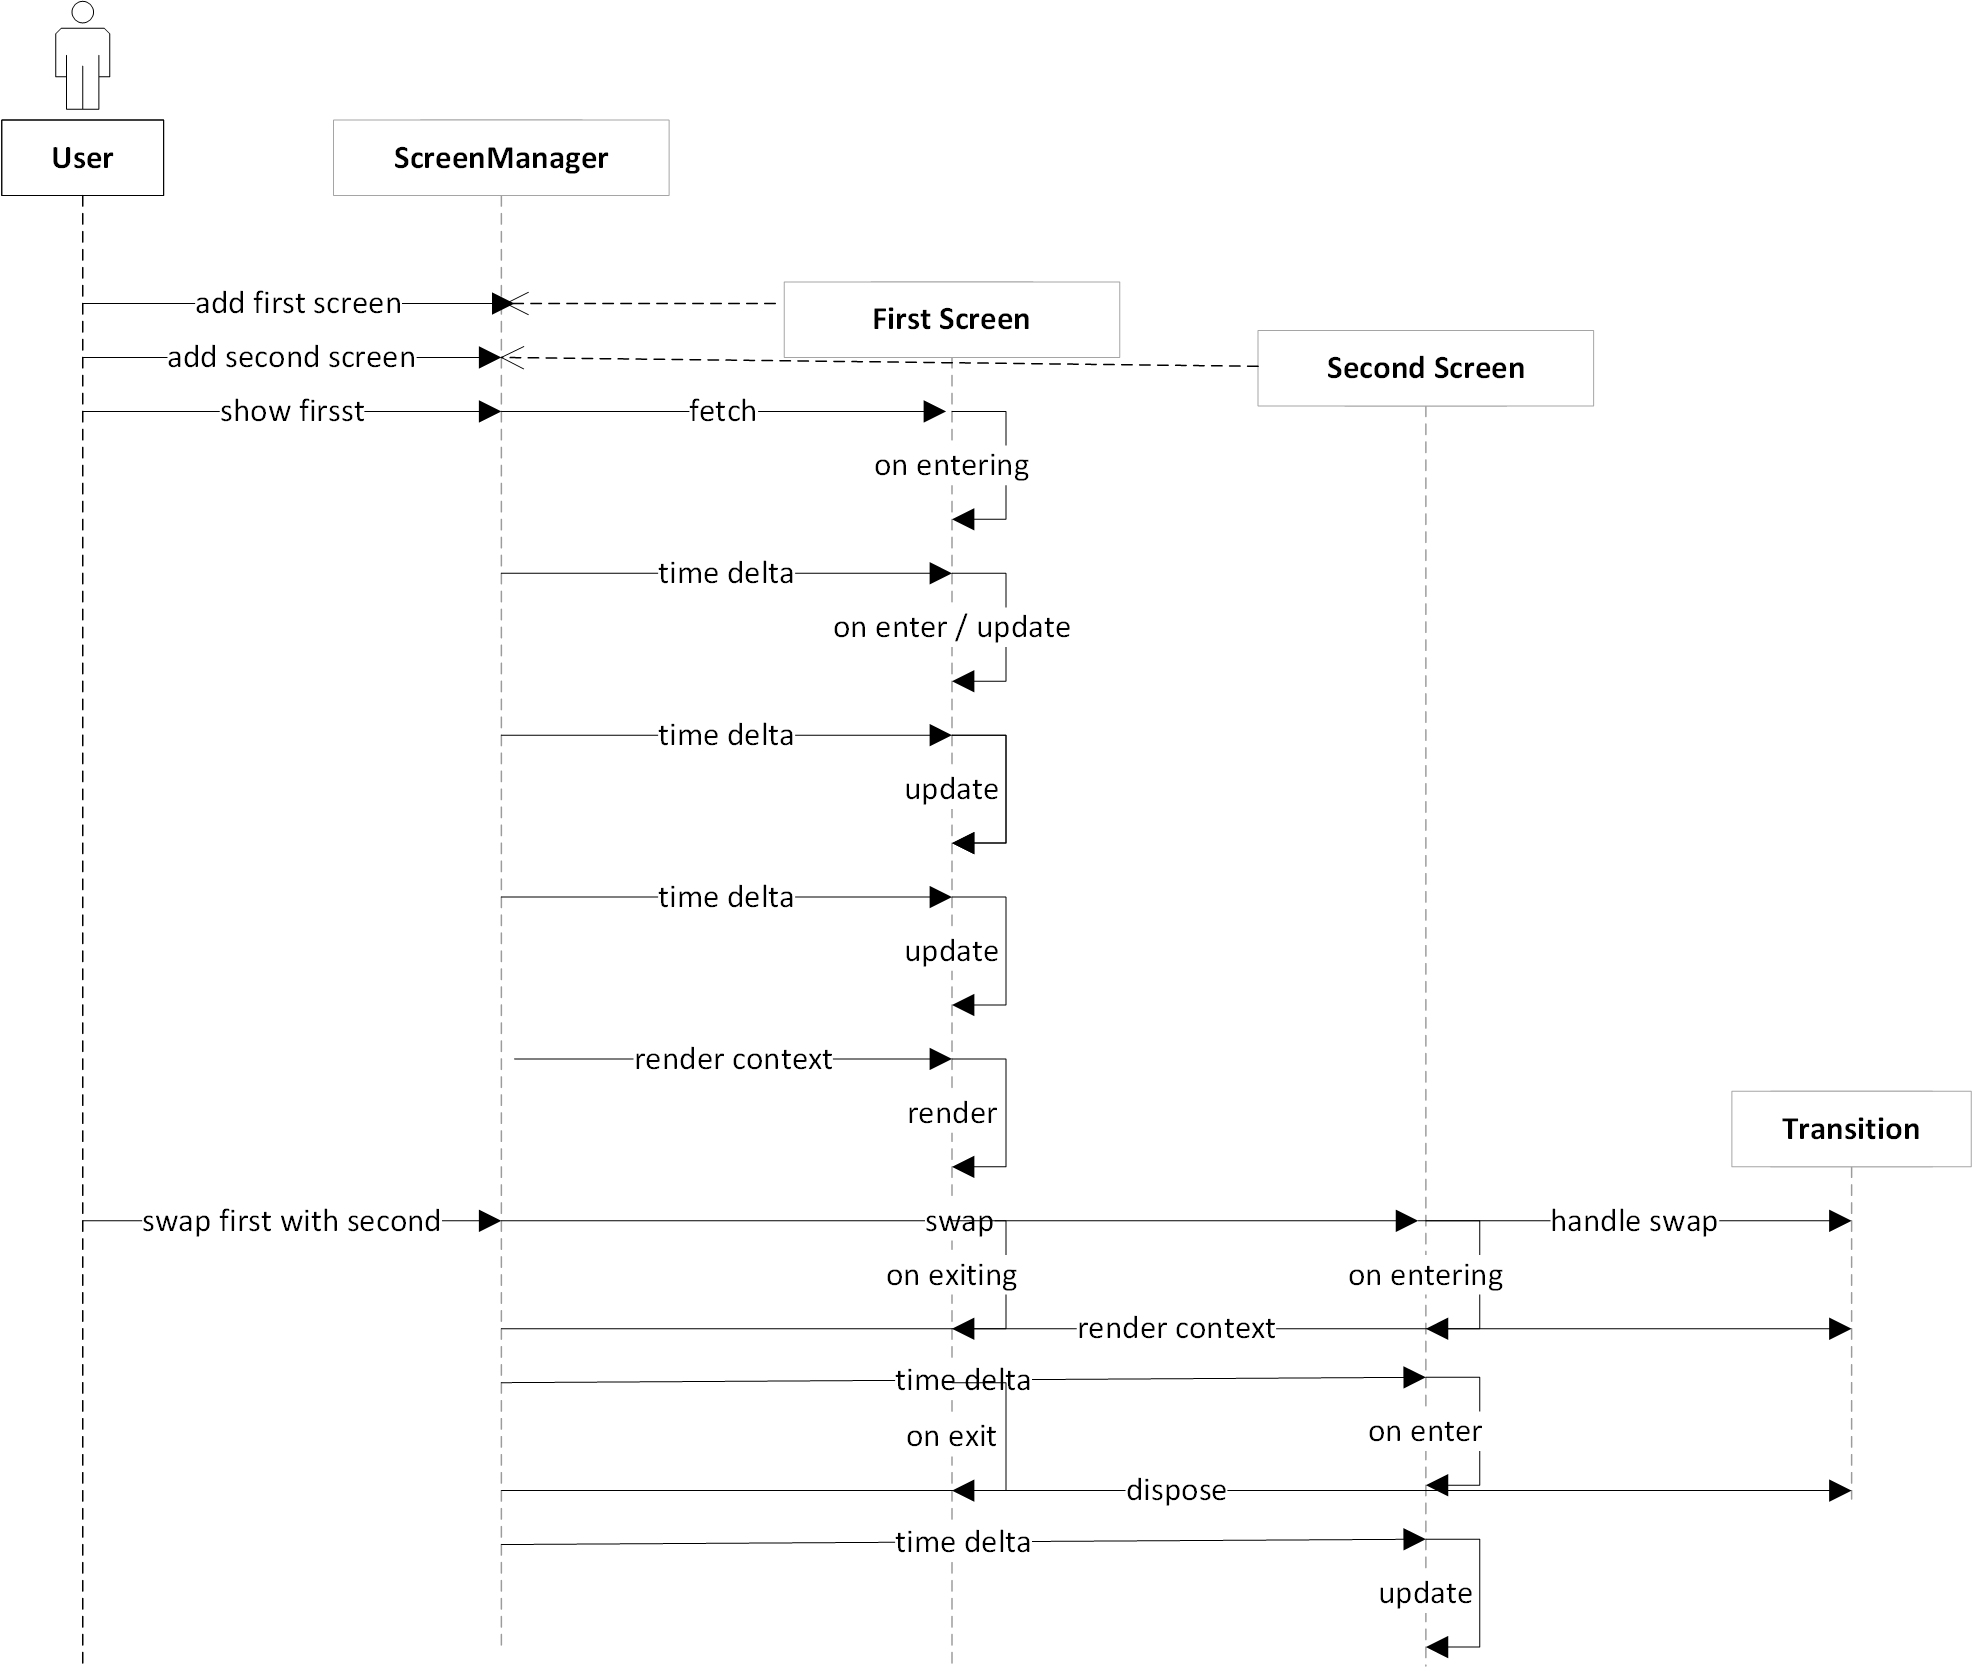
\includegraphics[width=165mm]{Images/screensystem_sequence}
		\caption{Διάγραμμα ακολουθίας του υποσυστήματος διαχείρισης οθονών}
		\label{fig:screensystem_sequence}
	\end{figure}	
	
	\subsection{Συστατικά του συστήματος}		
	\paragraph{Κεντρικό σύστημα διαχείρισης}
	Οι λειτουργίες του συστήματος διαχείρισης είναι οι παρακάτω:
	\begin{itemize}
	\item Απόδοση και ενημέρωσης 1-N σκηνών με δυναμικά εναλλασσόμενη σειρά στο πλαίσιο του κύκλου ζωής του πυρήνα.
	\item Προετοιμασία των οθονών και δυνατότητα εύρεσης χρησιμοποιώντας κλειδιά.
	\item Εύκολη προβολή, απόκρυψη, εναλλαγή οθονών χρησιμοποιώντας κλειδιά.
	\item Δυνατότητα εξατομίκευσης της απόδοσης κατά τις διάφορες μεταβάσεις των σκηνών.
	\end{itemize}

	\paragraph{Οικοδεσπότης οθόνης}
	Ο οικοδεσπότης οθόνης είναι υπεύθυνος για τα παρακάτω:
	\begin{itemize}
		\item Παραμετροποίηση συμβάντων κατά τις αλλαγές κατάστασης.
		\item Προσαρμοσμένη λογική και απόδοση .
		\item Εντολές αλλαγής κατάστασης.
		\item Εξατομίκευση απόδοσης κατά την εναλλαγή κατάστασης.
	\end{itemize}
	
	\paragraph{Εναλλαγή οθονών}
	Η εξατομίκευση και παραμετροποίηση της εναλλαγής οθονών λαμβάνει μέρος μέσα στο γενικό πλαίσιο απόδοσης οθονών. Ο εξατομικευτής αναλαμβάνει την απόδοση του screen buffer στον οποίο αποδόθηκε η οθόνη, την κατάσταση στην οποία βρίσκεται η οθόνη, την κατεύθυνση και το ποσοστό εξέλιξης της εναλλαγής. Ο εξατομικευτής περιγράφεται στο παράδειγμα κώδικα \ref{transition_delegate}.
			
	\lstset
	{
		style=sharpc, 
		caption={Εξατομικευτής εναλλαγής οθονών}
	}
	\begin{lstlisting}[label={transition_delegate}]	
delegate void TransitionRenderAction(ScreenState state, float progress, RenderTarget2D renderTarget, SpriteBatch batch);
	\end{lstlisting}
	
	\newpage
	\subsection{Αρχιτεκτονική}
Η αρχιτεκτονική του υποσυστήματος παρουσιάζεται στο \gls{UML} διάγραμμα. \ref{fig:core_screensystem}.
	\begin{figure}[h!]	
		\centering
		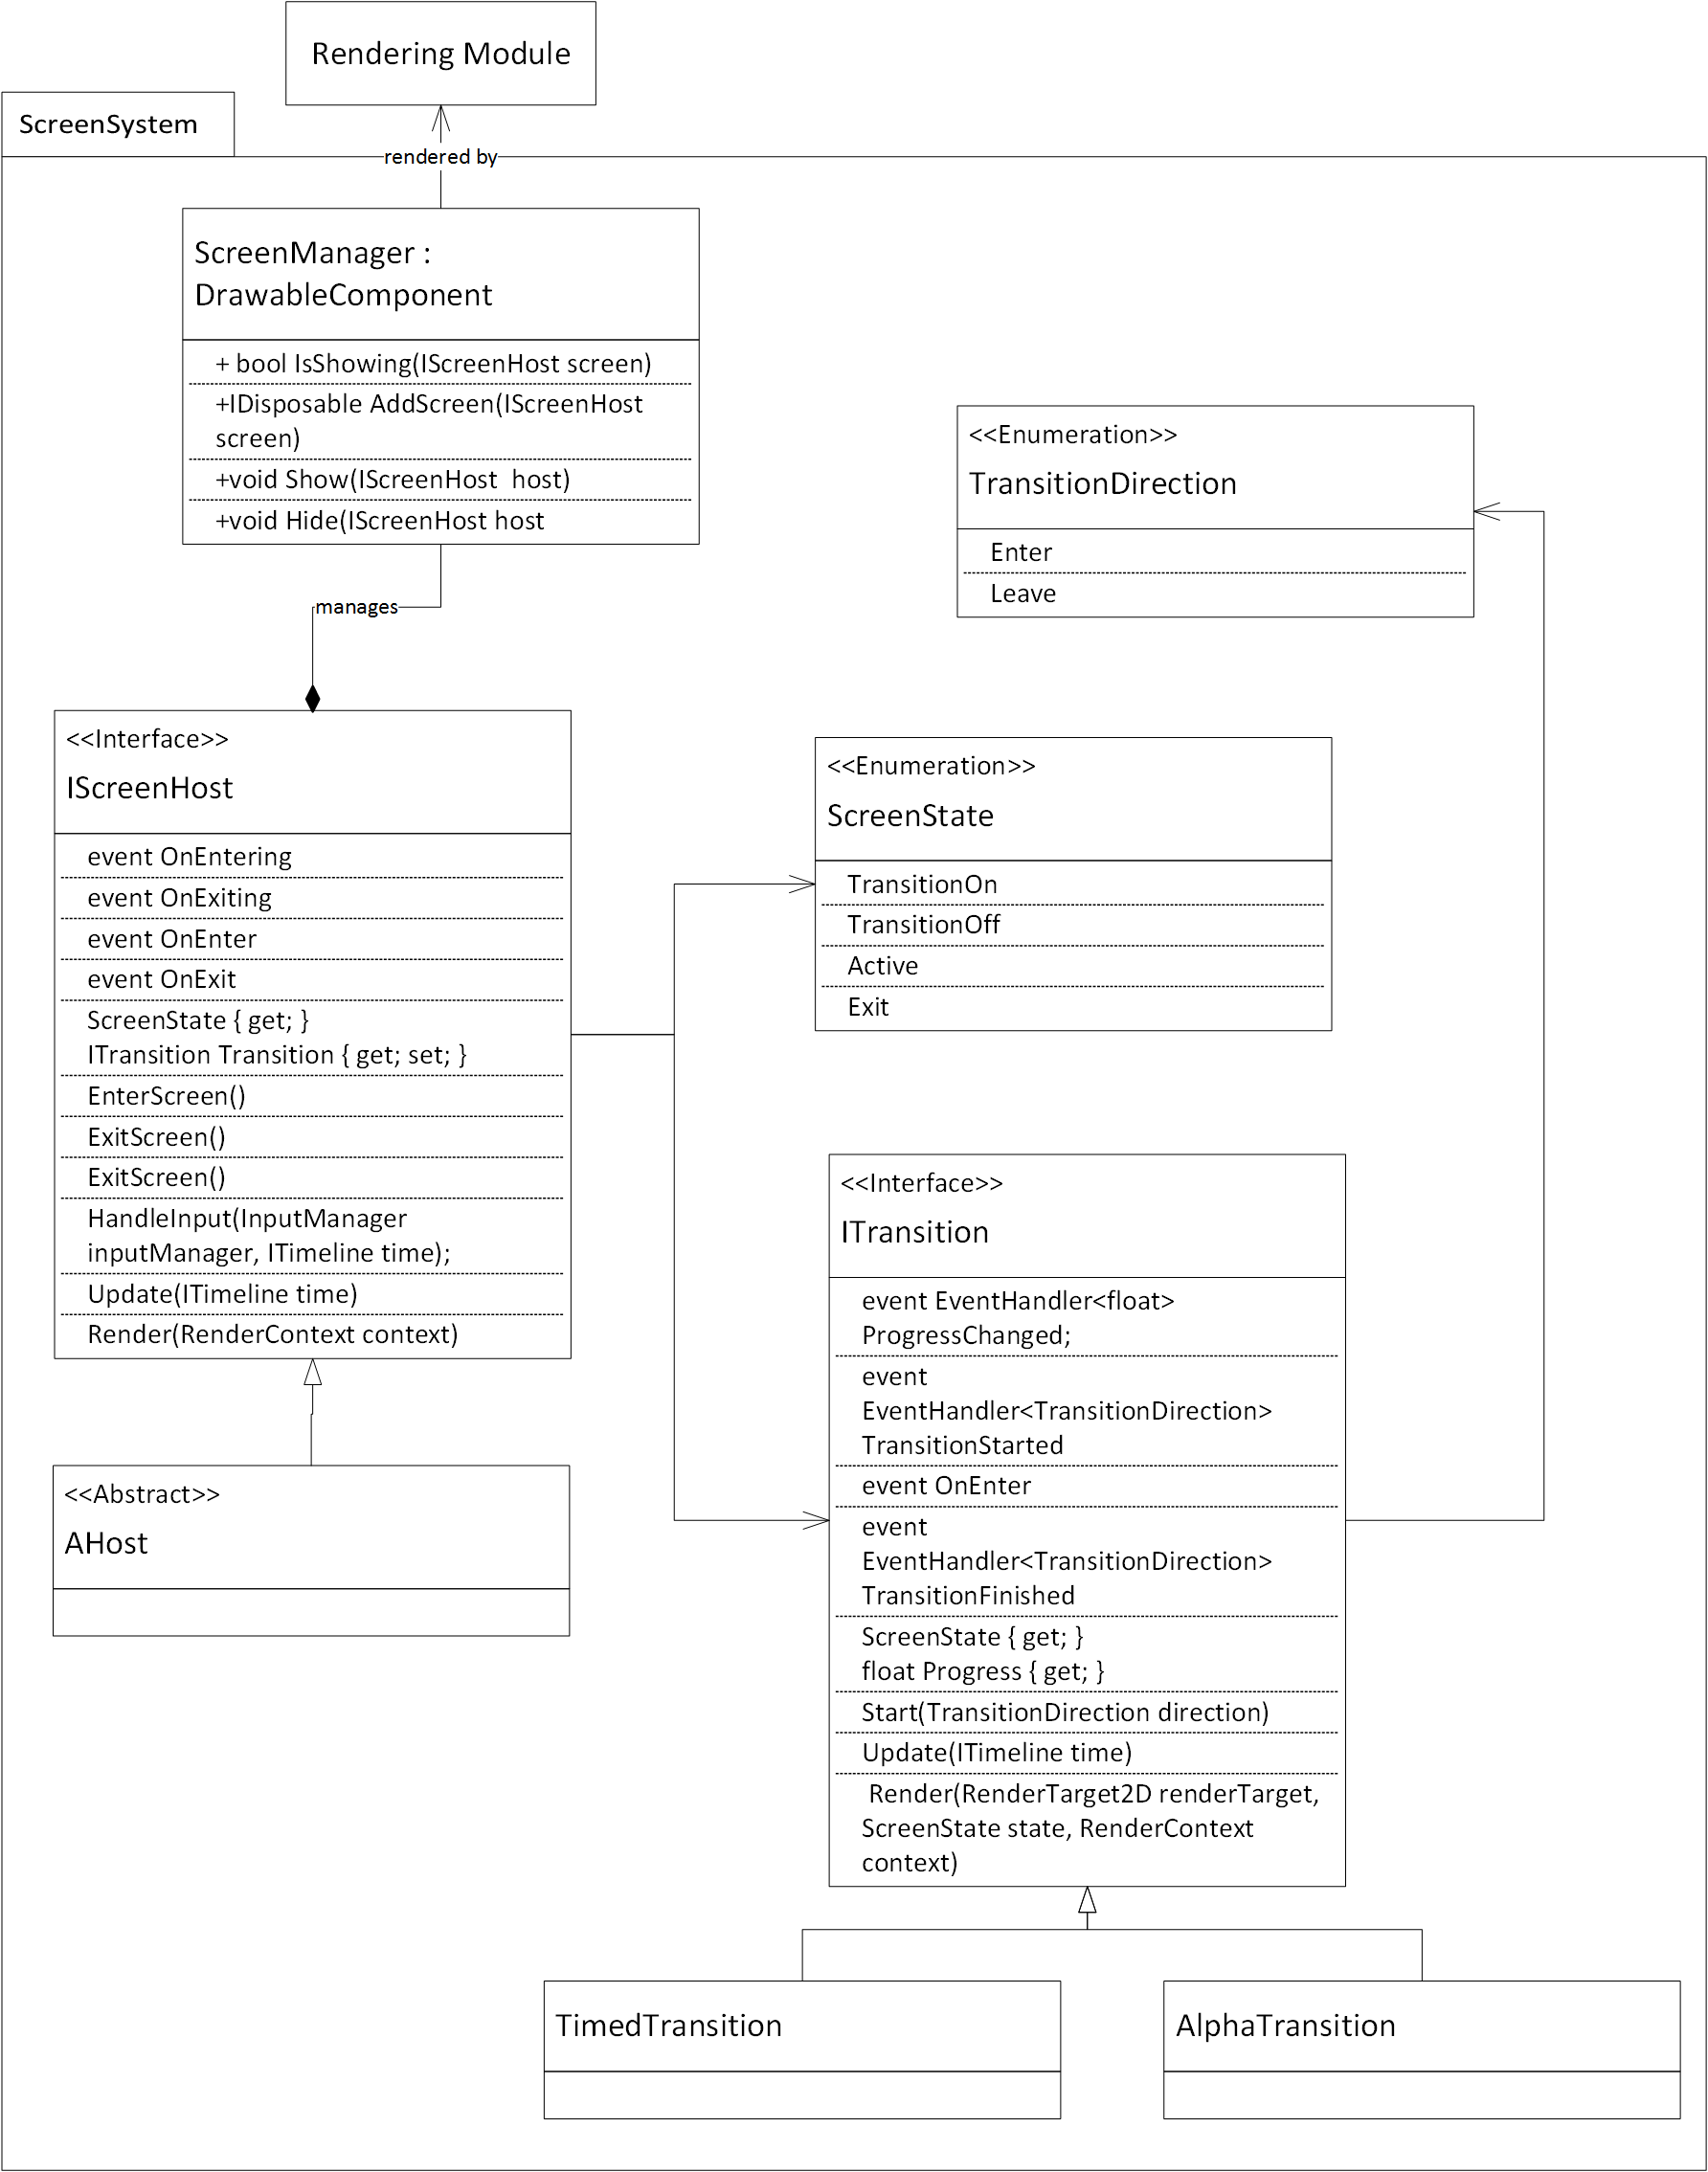
\includegraphics[width=160mm]{Images/core_screensystem}
		\caption{UML του υποσυστήματος διαχείρισης οθονών}
		\label{fig:core_screensystem}
	\end{figure}		
	
	\subsection{Παραδείγματα χρήσης API}

Στο παρακάτω παράδειγμα γίνεται καταχώριση μιας οθόνης-σκηνής στο υποσύστημα με κάποιο κλειδί. Στη συνέχεια το υποσύστημα εμφανίζει την σκηνή με εξατομικευμένη διαδικασία εναλλαγής.
	\lstset
	{
		style=sharpc, 
		caption={Παράδειγμα API του υποσυστήματος διαχείρισης οθονών-σκηνών}
	}
	\begin{lstlisting}
screenHost
.AddScreen(
	"FirstScreen",
	() => new MyFirstScreen());
		
screenHost["FirstScreen"]
.Show()
.Transition(
	Transition.WithTime(
         TimeSpan.FromSeconds(0.5),
         (state, progress, target, context) =>
         context.Batch.Draw(target, 
         (float)Math.Pow(progress - 1.0f, 2) * context.ScreenWidth, 
         Color.White * progress
    )
);
     
screenHost["FirstScreen"]
.Hide();   
	\end{lstlisting}
	
	\section{Σύστημα εισόδων}
	\subsection{Συσκευές ανθρώπινης διεπαφής}
	Η μηχανή πρέπει να είναι σε θέση να διαβάζει, να επεξεργάζεται και να χρησιμοποιεί συσκευές ανθρώπινης διεπαφής (human interface devices) \cite{gregory2009game}. Η διαδικασία ανάγνωσης χωρίζεται στις παρακάτω κατηγορίες:
	\begin{description}
	\item [Polling] Η κατάσταση κάποιον συσκευών (κυρίως της παλιάς σχολής) διαβάζεται ρωτώντας τη συσκευή για την κατάστασή της περιοδικά. Αυτό καταλήγει σε πλεονασμό, γιατί ρωτάει πολλές φορές χωρίς να παίρνει απάντηση, και πιθανών να συμβάλει σε μια μικρή καθυστέρηση, γιατί η αλλαγή κατάστασης μπορεί να γίνει μεταξύ ερωτήσεων.
	\item [Ιnterrupts (διακοπές)] Οι συσκευές στέλνουν δεδομένα μόνο όταν αλλάξει η κατάσταση με κάποιο τρόπο. Ο χρήστης μπορεί καταχωρίσει κώδικα σε συμβάντα ώστε να εκτελείται μόνο όταν συμβεί κάποια αλλαγή κατάστασης.
	\end{description}
	
	\subsection{Τύποι εισόδων}
	Οι διάφοροι τύποι εισόδων και οι πιθανές καταστάσεις τους είναι οι παρακάτω:
	\begin{description}	
	\item [Ψηφιακά κουμπιά] Tα ψηφιακά κουμπιά (digital buttons) έχουν δύο καταστάσεις: pressed / not pressed
	\item [Αναλογικοί άξονες και κουμπιά] Οι αναλογικοί άξονες και κουμπιά (analog axes and buttons) επιστρέφουν εύρος τιμών: το βαθμό της πίεσης της σκανδάλης ή τη θέση του μοχλού στο δισδιάστατο άξονα. 
	\item [Αναφορικοί άξονες] Οι αναφορικοί άξονες (relative axes) επιστρέφουν τιμές σε σχέση με το τελευταίο σημείο στο οποίο έγινε κάποια αλλαγή πχ το ποντίκι επιστρέφει τη διαφορά θέσης σε σχέση με το τελευταίο σημείο στο οποίο μετακινήθηκε.
	\item [Επιταχυντές] Οι επιταχυντές (accelerators) ανιχνεύουν τρισδιάστατες επιταχύνσεις.
	\item [Sensor bars] Αισθητήρες όπως οι κάμερες.
	\item [Αφή και χειρονομίες] Η αφή και χειρονομίες (touch and gestures) είναι τύποι εισόδου σε οθόνες αφής όπως στις οθόνες στα έξυπνα τηλέφωνα.
	\end{description}
	
	\subsection{Απαιτήσεις του υποσυστήματος διαχείρισης εισόδων}
	Η οντότητα θέλει να εκτελέσει κώδικα προσανατολισμένο κατά συμβάν εισόδου από συσκευή ανθρώπινης διεπαφής. Ο κώδικας αυτός εκτελείται αντίστοιχα για ποντίκι, πληκτρολόγιο και χειριστήριο. O χρήστης μπορεί να αλλάξει συσκευή διεπαφής ενώ βρίσκεται σε τρέχον παιχνίδι. Η βιβλιοθήκη δεν πρέπει να στηρίζεται σε κανένα υλικό ή συσκευή. Επίσης ο χρήστης χρειάζεται τη δυνατότητα να ακυρώνει συμβάντα.
		
	\subsection{Ακροατές}
	Το κάθε υποσύστημα διαχείρισης συσκευών ανθρώπινων διεπαφών αποτελείται από τον ακροατή (listener) για παράδειγμα τον MouseListener ή KeyboardListener, o οποίος χρησιμοποιεί τις βιβλιοθήκες του τρέχον λειτουργικού για την επιστολή συμβάντων των διεπαφών. Ανάλογα με την πλατφόρμα στην οποία αναπτύσσεται το παιχνίδι, δημιουργούνται οι αντίστοιχοι ακροατές μέσω του abstract factory \cite{Gamma:1995:DPE:186897}.
	Ο χρήστης μπορεί να προσκολλήσει κώδικα ο οποίος να εκτελείται ανά συμβάν π.χ. στη μετακίνηση του ποντικιού. Οι ακροατές κατά την καταχώρηση συμβάντος, επιστρέφουν ένα αντικείμενο το οποίο μπορεί να χρησιμοποιηθεί για την κατάργησή του καταχωρημένου συμβάντος. Οι ακροατές ανάλογα με τις επιλογής επιστολής, όπως το δέλτα του χρόνου επιστολής συμβάντος διπλού click είναι 200ms, αποστέλλουν τα συμβάντα στους καταχωρημένους εκτελεστές. Το κεντρικό σύστημα διαχείρισης εισόδου ενημερώνει όλες τις συνδεδεμένες συσκευές εισόδου. 
	Ο εκτελέσιμος κώδικας μπορεί να γραφτεί μια φορά, ανεξαρτήτως συμβάντος, και να προσκολληθεί στην προετοιμασία του κύκλου ζωής σε υποσυστήματα διεπαφών. Επίσης με τη χρήση των active binders, μπορεί να γίνει απενεργοποίηση των ακροατών π.χ. όταν είναι ανοιχτό το menu επιλογών, οι o ActiveBinder του παιχνιδιού είναι απενεργοποιημένος, με αποτέλεσμα τα συμβάντα τα οποία είναι προσκολλημένα στον διαχειριστή εισόδων να μην εκτελούνται. Στο \gls{UML} διάγραμμα \ref{fig:core_input} παρουσιάζεται η αρχιτεκτονική του υποσυστήματος.
	
	
	\begin{figure}[h!]
		\centering
		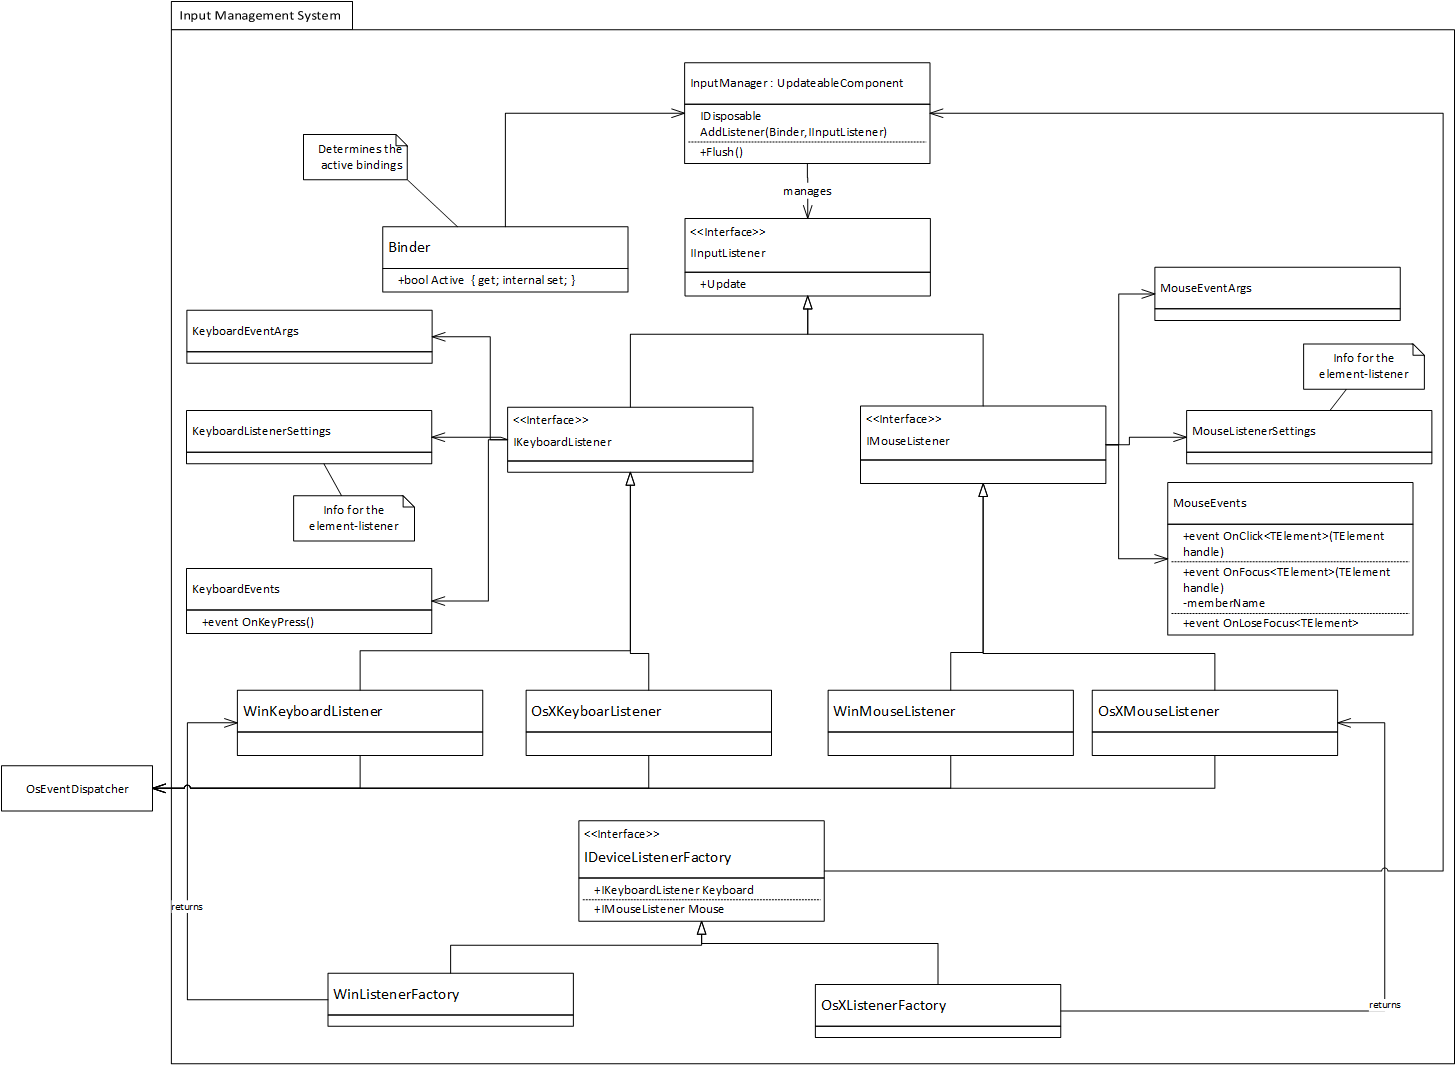
\includegraphics[width=165mm]{Images/core_input}
		\caption{Αρχιτεκτονική υποσυστήματος διαχείρισης εισόδων}
		\label{fig:core_input}
	\end{figure}
		
	\newpage
	Στο παράδειγμα κώδικα \ref{cs:listeners} παρουσιάζεται η δημιουργία και καταχώρηση των ακροατών. 
	\lstset
	{		
		style=sharpc, 
		caption={Παράδειγμα καταχώρησης ακροατών στο υποσύστημα εισόδων},
	}
	\begin{lstlisting}[label=cs:listeners]
inputManager.AddListener(
ingameBinder,
factory => factory.GamepadListener
{
	Settings = MouseSettings
		    .DoubleClickDelta(Timespan.FromSeconds(0.2))
			.DragDelta(Timespan.FromSeconds(0.2)),
	Events   = MouseEvents
	        .OnLeftClick(sender,args) => this.Shoot())
	        .OnLeftDoubleClick(sender,args) => this.Roll())      	
});

inputManager.AddListener(
ingameBinder,
factory => factory.GamepadListener
{
	Settings = GamepadSettings.Default,
	Events   = GamepadEvents
			.OnXButtonPress(sender,args) => this.Shoot())
			.OnYButtonPress(sender,args) => this.Roll())      	
});
\end{lstlisting}

\section{Φυσική και εντοπισμός συγκρούσεων}
Η φυσική στα παιχνίδια έχει ως βάση τα μαθηματικά. Η ανάλυση του συστήματος της φυσικής επικεντρώνεται σε μοντελοποίηση υψηλού επιπέδου. Η υλοποίησή του βασίζεται στην υλοποίηση μαθηματικών λειτουργιών γεωμετρίας, γραμμικής άλγεβρας και κινηματικής.

\subsection{Τα παιχνίδια ως soft real-time simulations}
Οι επιστήμονες αποκαλούν τα παιχνίδια soft real-time interative agent-based computer simulations.
Στα περισσότερα παιχνίδια ένα υποσύστημα του πραγματικού κόσμου μοντελοποιείται μαθηματικά, ώστε να μπορεί να αναπαραχθεί και να χειριστεί από τον υπολογιστή. 
Ενα agent-based simulation είναι μια προσομοίωση η οποία περιγράφει πώς αλληλεπιδρούν τα διάφορα αντικείμενα και χαρακτήρες μέσα στον κόσμο.
Όλα τα αλληλεπιδραστικά παιχνίδια είναι temporal simulations δηλαδή το μοντέλο του εικονικού κόσμου είναι δυναμικό, αλλάζει με την πάροδο του χρόνου, με βάση τα διάφορα συμβάντα και την εξέλιξη της ιστορίας.
Όλα simulations και η επικοινωνία του παιχνιδιού με τον χρήστη γίνεται σε πραγματικό χρόνο (interactive real-time simulations. 

Στον πυρήνα όλων τον συστημάτων πραγματικού χρόνου υπάρχει το "at least 24 fps deadline" δηλαδή για να δημιουργείται η ψευδαίσθηση της κίνησης, η οθόνη θα πρέπει να ανανεώνεται τουλάχιστον 24 φορές το δευτερόλεπτο. Φυσικά υπάρχουν και άλλα είδη προθεσμιών (deadlines). Για να θεωρείται η προσομοίωση φυσικής σταθερή, πρέπει να ενημερώνεται τουλάχιστον 120 φορές το δευτερόλεπτο, ο μηχανισμός τεχνητής νοημοσύνης θα πρέπει να καλείται τουλάχιστον κάθε δευτερόλεπτο και οι buffers ήχου 60 φορές το δευτερόλεπτο για να αποτρέπονται δυσλειτουργίες του συστήματος διαχείρισης ήχου.

Ένα soft real time system είναι ένα σύστημα στο οποίο χαμένες ενημερώσεις δεν είναι καταστροφικές.
Τα μαθηματικά μοντέλα τα οποία απαρτίζουν το σύστημα μπορεί να είναι είτε αριθμητικά είτε αναλυτικά. Τα αριθμητικά μοντέλα μπορούν να αξιολογηθούν για κάθε τιμή της ανεξάρτητης μεταβλητής ενώ οι τιμές του αναλυτικού μοντέλου καθορίζονται διακριτά κατά τη διάρκεια της προσομοίωσης και είναι πιο συχνά γιατί η επόμενη κατάσταση της προσομοίωσης καθορίζεται από την εισαγωγή δεδομένων σε πραγματικό χρόνο από το χρήστη. \cite{realtime_collision04}

\subsection{Βασικές έννοιες φυσικής του συστήματος}
Οι οντότητες της φυσικής έχουν τις παρακάτω ιδιότητες για τη προσομοίωσή τους στο υποσύστημα φυσικής.

\begin{description}
\item [Μάζα] Η μάζα (mass) στη φυσική συνδέεται με δύο έννοιες, την αδράνεια της μεταφορικής κίνησης και τη βαρύτητα. Η μάζα είναι μια ορισμένη ποσότητα η οποία χρησιμοποιείται για την περιγραφή ενός συστήματος.

\item [Πυκνότητα]  Η πυκνότητα (density) εκφράζει τη μάζα του υλικού που περιέχεται σε μία μονάδα όγκου. 

\item [Force] Σε ότι αφορά τα ελεύθερα σώματα, η δύναμη (force) είναι γενικά η αιτία μεταβολής της κινητικής τους κατάστασης, δηλαδή αυτή που τα επιταχύνει ή τα επιβραδύνει. Αυτό ισχύει και για την περιστροφή τους, που μπορεί να επιταχυνθεί ή να επιβραδυνθεί. Για σώματα που δεν είναι ελεύθερα να κινηθούν με όλους τους τρόπους, αυτά δηλαδή που είτε είναι αναρτημένα κάπου και μπορούν να κινηθούν μόνο γύρω από σημείο ή άξονα ή σε προκαθορισμένη τροχιά, καθώς και σε όσα εφαρμόζονται δυνάμεις τριβής ή γενικά αντιδράσεις στήριξης.

\item [Ροπή] Ροπή (torque) δυνάμεως ως προς σημείο είναι το διανυσματικό φυσικό μέγεθος που έχει μέτρο ίσο προς το γινόμενο της δύναμης επί την (κάθετη) απόσταση της δύναμης από το σημείο. Κατά όμοιο τρόπο ροπή δυνάμεως ως προς άξονα είναι το διανυσματικό μέγεθος που έχει ως μέτρο το γινόμενο της δύναμης επί την (κάθετη) απόσταση της δύναμης από τον άξονα, και φορέα τον άξονα.

\item [Ώθηση] Η ώθηση (impulse) είναι το φυσικό μέγεθος που ισοδυναμεί με την μεταβολή της ορμής ενός σώματος στο οποίο εφαρμόζεται μία δύναμη για κάποιο χρονικό διάστημα. Ισούται με το γινόμενο της δύναμης που ασκείται στο σώμα επί τον συνολικό χρόνο εφαρμογής της

\item [Restitution] Το law of restitution δηλαδή ανάκτηση με βάση το κέρδος. Η υποχρέωση της οντότητας να αποζημιώσει από τα κέρδη τη για κάποιο γεγονός. 

\item [Απόσβεση] Η απόσβεση (damping), είναι η επιρροή εντός η κατά ενός συστήματος ταλάντωσης που έχει ως αποτέλεσμα τη μείωση, τον περιορισμό η την πρόληψη των ταλαντώσεών του. Σε φυσικά συστήματα , απόσβεση παράγεται με διαδικασίες που διαχέουν την ενέργεια που αποθηκεύεται στο ταλάντωση.
\end{description}

\subsection{Οντότητες του συστήματος}

Οι οντότητες που απαρτίζουν το υποσύστημα φυσικής είναι οι παρακάτω:

\begin{description}
\item [Shape]
Ένα αντικείμενο το οποίο αντιπροσωπεύει ένα γεωμετρικό σχήμα όπως κύκλο, πολύγωνο κλπ
\item [World]
Η συλλογή των bodies, fixtures και constraints και η λογική της αλληλεπίδρασής τους.
\item [World Solver]
Ο solver αναλύει την προσομοίωση και εκτελείται ανεξάρτητα από το χρόνο εκτέλεσης του προγράμματος.
\item [Fixture]
To fixture δένει ένα body με ένα shape και προσθέτει επιπλέον ιδιότητες όπως πυκνότητα, τριβή και αποκατάσταση. Το fixture εντάσσει ένα σχήμα στο σύστημα συγκρούσεων ώστε να αλληλεπιδρά με τα υπόλοιπα σχήματα στον κόσμο.
\item [Body] 
To body περιέχει της πληροφορίες ενός αντικειμένου του οποίου δεν βλέπεις ούτε συγκρούεσαι και έχει τις παρακάτω ιδιότητες:
	\begin{description}
		\item [Mass] To βάρος
		\item [Velocity] η ταχύτητα και η κατεύθυνση της κίνησης υπό μορφή διανύσματος.
		\item [Rotation inertia] πόσος κόπος χρειάζεται για να ξεκινήσει η περιστροφή ή η κίνηση
		\item [Angular velocity] πόσο γρήγορα και σε ποια κατεύθυνση περιστρέφεται
		\item [Position] που βρίσκεται στο σύστημα καρτεσιανών συντεταγμένων
		\item [Angle] υπό ποια γωνία βρίσκεται
	\end{description}
Οι τύποι των bodies είναι:
	\begin{description}
		\item [Static]
		Στατικά στο σύστημα συντεταγμένων. Δεν ανταποκρίνεται σε εξωτερικές δυνάμεις.
		\item [Dynamic]
		Είναι μέρος του συστήματος συγκρούσεων. Ανταποκρίνεται σε εξωτερικές δυνάμεις και κανονικά σε όλες τα μέρη της προσωμοίωσης.
		\item [Kinematic] 
		Κινείται ανάλογα με το προκαθορισμένο script ταχύτητας. Δεν ανταποκρίνεται σε εξωτερικές δυνάμεις.
	\end{description}
\item [Constraint]
Περιορισμός κατά την προσομοίωση του body.
\item [Joint] 
Το joint συνδέει δύο ή περισσότερα bodies μεταξύ τους.
\item [Joint Motor]
Ο οδηγός της κίνησης των συνδεδεμένων με joint bodies. 
\item [Joint Limit]
Το joint limit περιορίζει το εύρος κίνησης του joint motor.
\end{description}

\subsection{Αρχιτεκτονική}
Οι σχέσεις μεταξύ των οντοτήτων παρουσιάζονται στο διάγραμμα \ref{fig:physics_abstract}
	\begin{figure}[h!]
		\centering
		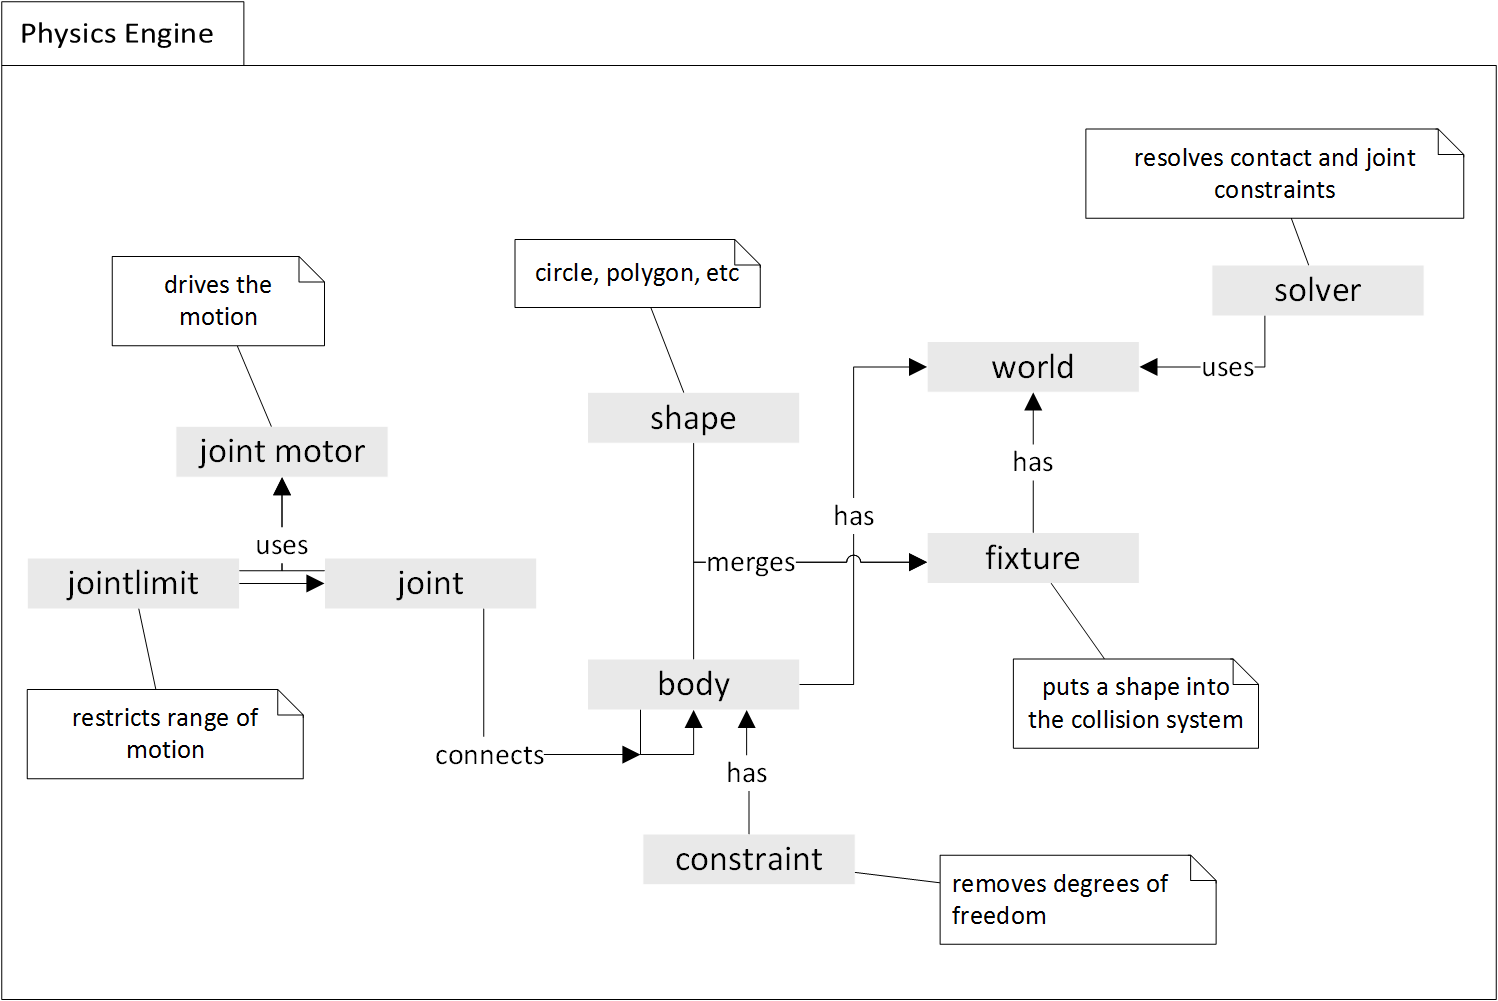
\includegraphics[width=165mm]{Images/physics_overview}
		\caption{Υποσύστημα φυσικής και εντοπισμού συγκρούσεων}
		\label{fig:physics_abstract}
	\end{figure}
	
\section{Διεπαφή χρήστη}
Η επικοινωνία του χρήστη με τη μηχανή γίνεται συνήθως με συσκευές ανθρώπινης διεπαφής. Η επικοινωνία αυτή αντί να περιορίζεται σε ένα απλό σήμα εισόδου (input signal), μπορεί να γίνει εύκολα, αυτονόητα, αποτελεσματικά και φιλικά προς το χρήστη. Διεπαφή χρήστη (user interface) ονομάζουμε το σύνολο γραφικών στοιχείων, τα οποία εμφανίζονται στην οθόνη κάποιας ψηφιακής συσκευής (π.χ. Η/Υ) και χρησιμοποιούνται για την αλληλεπίδραση του χρήστη με τη συσκευή αυτή. Παρέχει ενδείξεις και εργαλεία μέσω γραφικών, προκειμένου ο χρήστης να φέρει εις πέρας κάποιες επιθυμητές λειτουργίες.

\subsection{Απαιτήσεις}
Κατά το σχεδιασμό ενός παιχνιδιού συχνά δημιουργείται η ανάγκη για επικοινωνία με τον παίχτη μέσω διεπαφή χρήστη. Η δομή του, το στυλ της απόδοσης (χρώμα, textures, fonts κλπ),η απόδοση (rendering), η συμπεριφορά και ο εκτελέσιμος κώδικας κατά τα συμβάντα της διεπαφής πρέπει να είναι αποσυνδεδεμένα έτσι ώστε να μην επηρεάζει το ένα το άλλο. Επίσης η διεπαφή χρήστη προορίζεται για διάφορες αναλύσεις οθόνης και \Gls{DPI}. Μια καλή στρατηγική στην κατανόηση και επίλυση προβλημάτων είναι η εύρεση παρόμοιων και σχετικών προβλημάτων. Στο σχεδιασμό ιστοσελίδων η HTML χρησιμοποιείται και τη δομή της σελίδας, το CSS για το στυλ και η Javascript για τη συμπεριφορά.

\subsection{Δομή στη μνήμη}	
Όταν ζητηθεί από τον περιηγητή (browser) να φορτώσει μια ιστοσελίδα στη μνήμη από κάποιον web server, o περιηγητής αναλύει το html αρχείο και οργανώνει τα στοιχεία στη μνήμη σε δομή δέντρου \gls{B-Tree}. Λόγω της οργάνωσης σε δέντρο, δημιουργούνται σχέσεις μεταξύ των στοιχείων.

	\begin{figure}[h!]
		\centering
		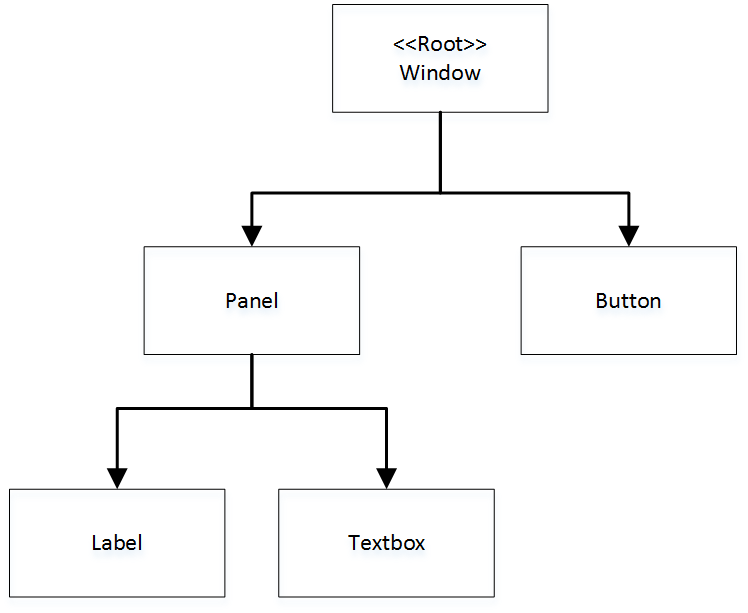
\includegraphics[width=90mm]{Images/ui_btree}
		\caption{B-Tree διεπαφής χρήστη}
		\label{fig:ui_b-tree}
	\end{figure}
	
Στο παράδειγμα \ref{fig:ui_b-tree}  το window είναι η ρίζα (root) του δέντρου. Το window έχει δύο παιδιά, ένα panel και ένα button. Το button έχει και αυτό δύο παιδιά: ένα textbox και ένα label. Τα button, textbox και label είναι leaves (φύλλα) του δέντρου, το panel είναι κόμβος (node), και το panel και button αδέλφια (siblings).

\paragraph{Πλεονεκτήματα της οργάνωσης σε B-Tree}
Η οργάνωση σε \gls{B-Tree} έχει τα παρακάτω πλεονεκτήματα:
\begin{description}
	\item [Ευκολία κατά την απόδοση στην οθόνη] Λόγω της συγκεκριμένης δομής, τα στοιχεία μπορούν να στοιχηθούν και να αποδοθούν ανάλογα με τη σχέση τους με συγγενικά στοιχεία. Καθώς διαβαίνεται (traversing) το δέντρο, το κάθε στοιχείο αποδίδεται σε πιο πάνω επίπεδο μέσα στο πλαίσιο του πατέρα, δηλαδή το στοιχείο παιδί βρίσκεται "πάνω" από τον πατέρα, ούτως ώστε να δημιουργείται η ψευδαίσθηση του βάθους.
	\item [Καλύτερη απόδοση στην οθόνη] Όταν κάποιος κόμβος δεν διατέμνεται με το πλαίσιο του παράθυρου, δεν αποδίδεται στην οθόνη και η διάβαση του δέντρου σταματά.
	\item [Αποσαφήνιση σειράς συμβάντων] Κατά τα συμβάντα στη διεπαφή χρήστη, ένα πλαίσιο μπορεί να καλύπτει περισσότερα από ένα συμβάντα. Ένα στοιχείο έχει τεμνόμενα πλαίσια όταν οποίο βρίσκεται μέσα σε ένα άλλο στοιχείο. To συμβάν γίνεται στο στοιχείο το οποίο βρίσκεται τελευταίο στην ιεραρχία.
	\item [Προχωρημένη και γρήγορη επιλογή στοιχείων] Η επιλογή των στοιχείων γίνεται με προχωρημένα κριτήρια, όπως τη σχέση ενός στοιχείου με συγγενικά στοιχεία στη δομή, και σε λογαριθμικό χρόνο.
	
Στο \gls{UML} διάγραμμα \ref{fig:ui_structure} παρουσιάζεται το υποσύστημα το οποίο είναι υπεύθυνο για το κτίσιμο της δομής της διεπαφής χρήστη στη μνήμη.
\end{description}
	\begin{figure}[h!]
		\centering
		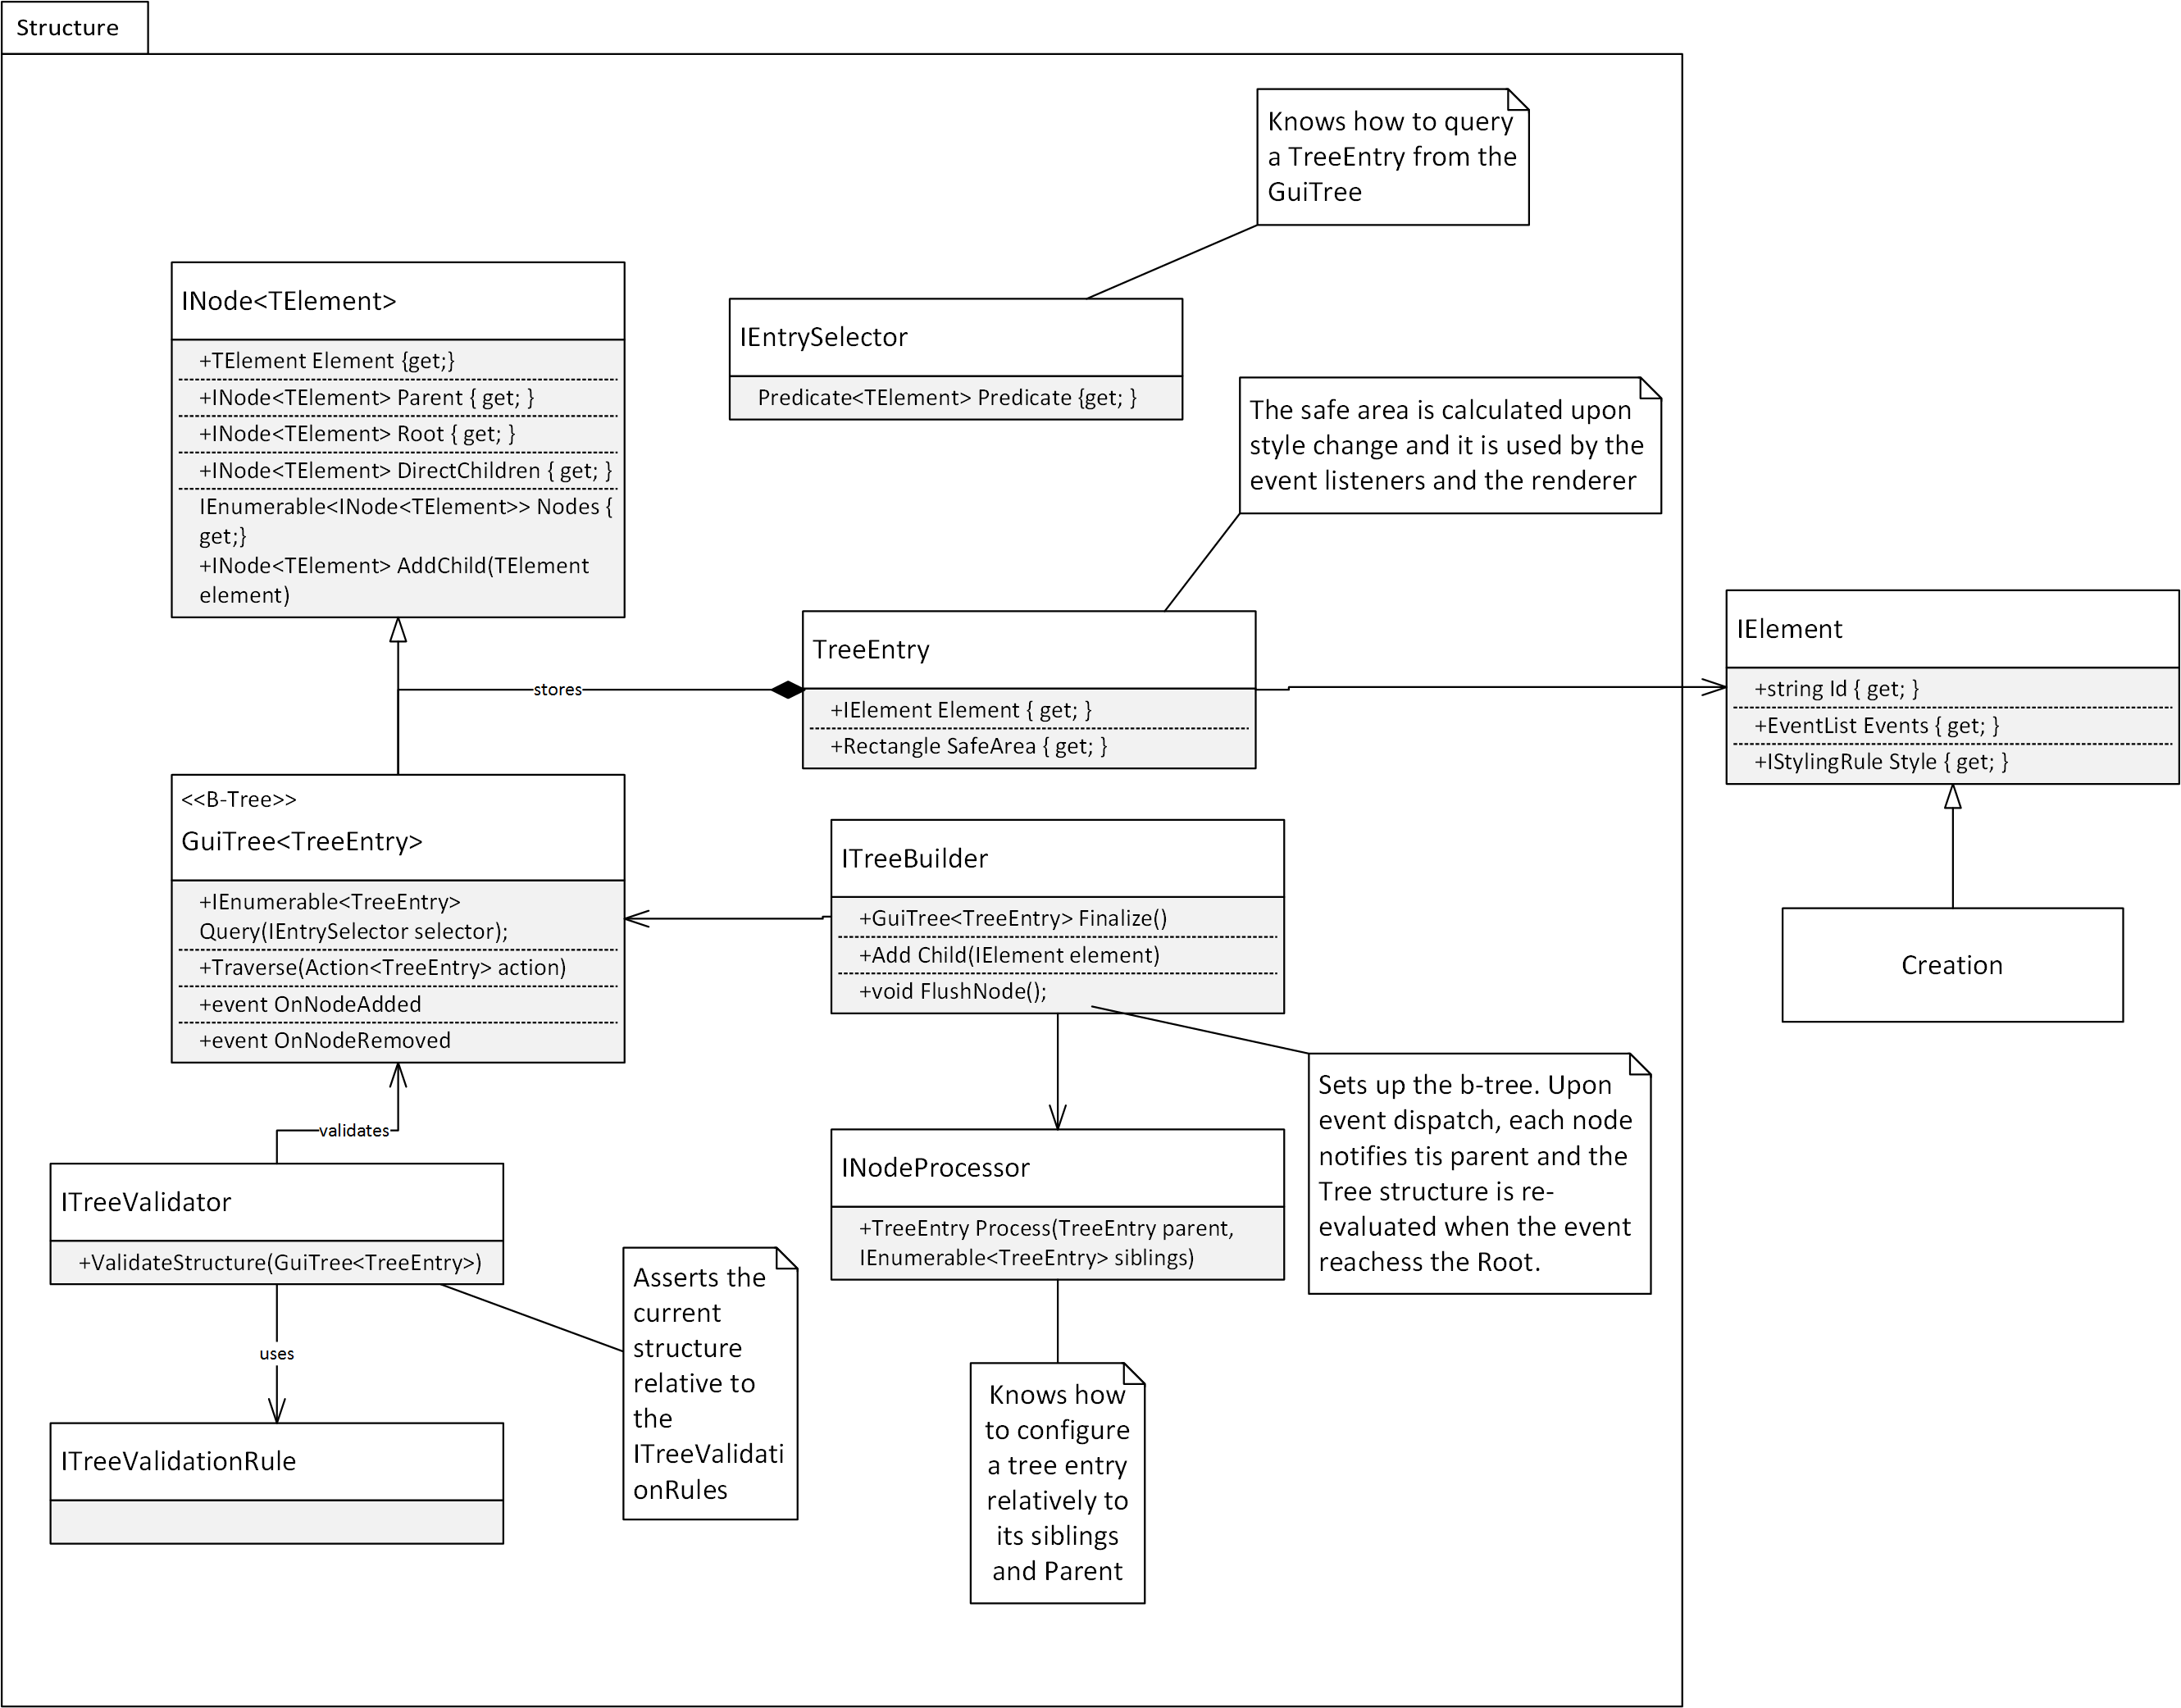
\includegraphics[width=165mm]{Images/gui_structure}
		\caption{Δομή διεπαφής χρήστη}
		\label{fig:ui_structure}
	\end{figure}

\subsection{Τα υποσυστήματα διεπαφής χρήστη}	
Το σύστημα διεπαφής χρήστη χωρίζεται στα παρακάτω υποσυστήματα
	\begin{description}
		\item [Οργάνωσης δομής] Το υποσύστημα οργάνωσης δομής αναλαμβάνει το κτίσιμο και την αποθήκευση της ιεραρχίας των στοιχείων στη μνήμη.
		\item [Style definition] Το style definition οποίο εμπλουτίζει την απόδοση με animations, textures κλπ.
		\item [Factory] Μέσω του factory o οποίο ο χρήστης της μηχανής δημιουργεί στοιχεία. Το υποσύστημα αυτό χρησιμοποιεί το abstract factory pattern \cite{Gamma:1995:DPE:186897} για δημιουργία στοιχείων ανεξαρτήτου πλατφόρμας, και fluent builder για τη δημιουργία στοιχείων με φιλικό στον χρήστη \gls{API}.
	\end{description}
	
Οι σχέσεις μεταξύ των υποσυστημάτων του συστήματος διεπαφής χρήστη παρουσιάζονται στο \gls{UML} διάγραμμα \ref{fig:ui_system}.
	\begin{figure}[h!]
		\centering
		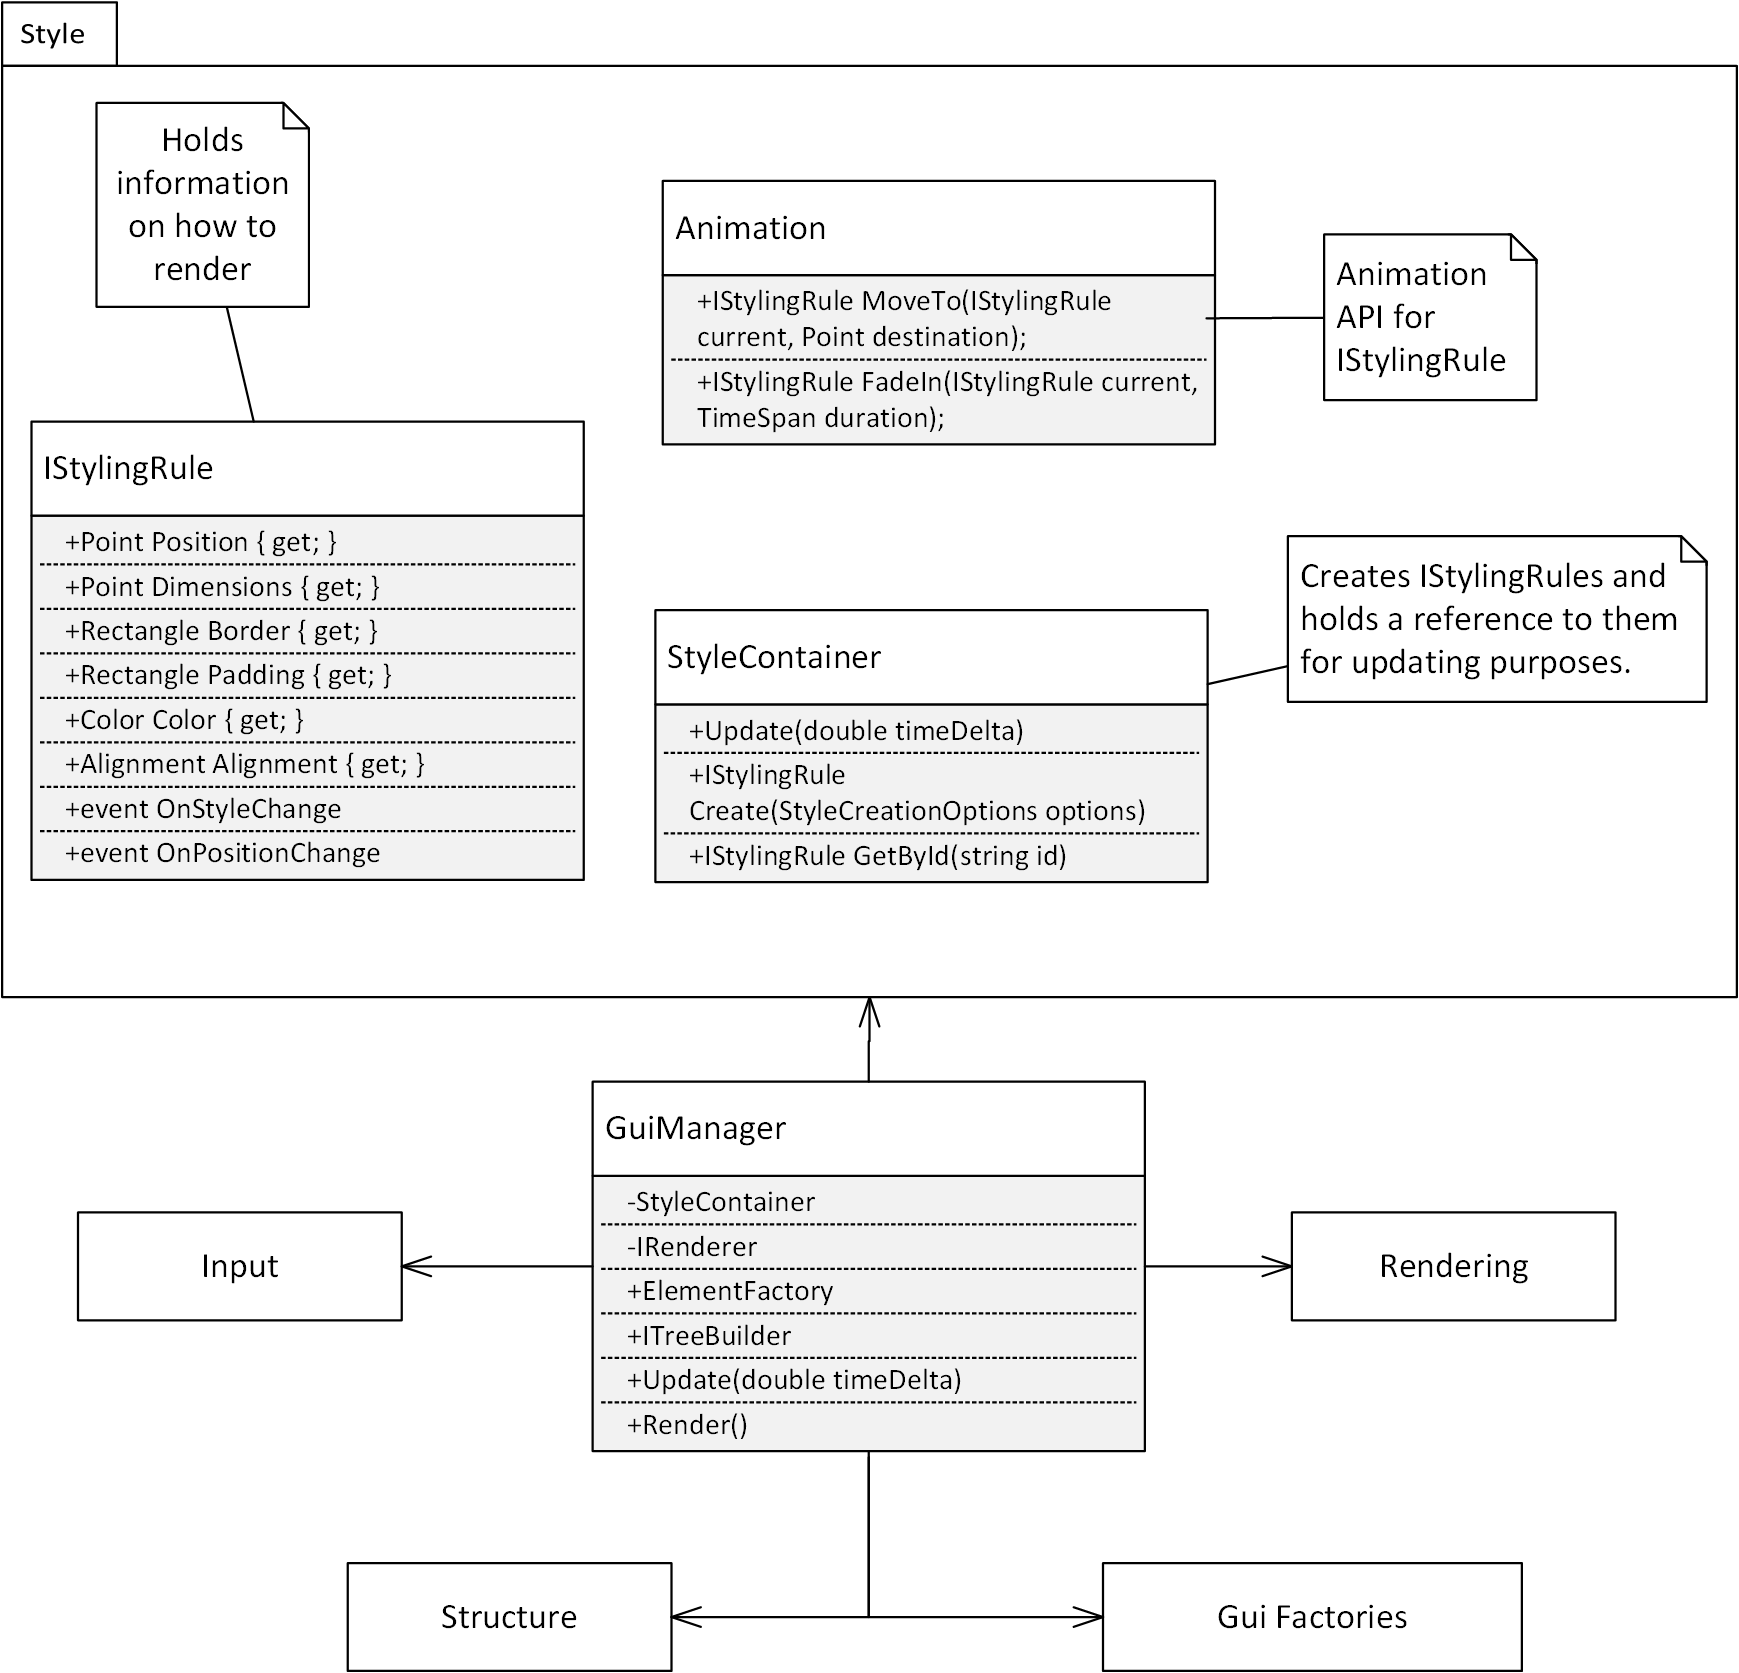
\includegraphics[width=165mm]{Images/gui_system}
		\caption{UML του συστήματος ανθρώπινης διεπαφής}
		\label{fig:ui_system}
	\end{figure}	
	
\newpage
\subsection{Κύκλος ζωής διεπαφής χρήστη}
Η σειρά προετοιμασίας διαμόρφωσης και παρουσίασης της διεπαφής χρήστη φαίνεται στο διάγραμμα \ref{fig:ui_usage}.

\begin{figure}[h!]
	\centering
	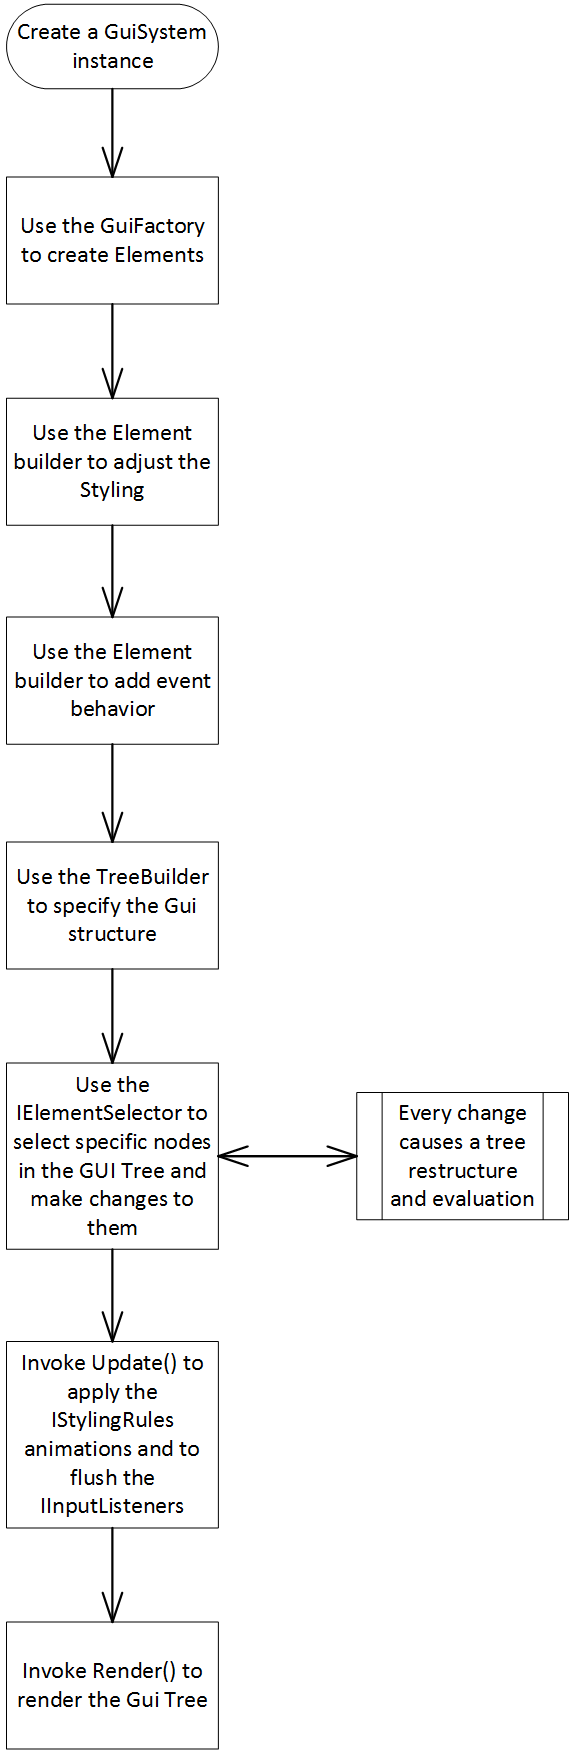
\includegraphics[width=130mm]{Images/gui_usage}
	\caption{Κύκλος ζωής διεπαφής χρήστη}
	\label{fig:ui_usage}
\end{figure}
\newpage

\section{Διαχείριση πόρων}
Τα παιχνίδια απαρτίζονται από πολλά είδη δεδομένων, είτε αυτά είναι τρισδιάστατα μοντέλα, textures, αρχεία ήχου κλπ. Η μηχανή πρέπει να είναι σε θέση να φορτώνει στη μνήμη και να αφαιρεί αυτά τα δεδομένα δυναμικά. Χρειάζεται λοιπόν κάποιου είδους διαχειριστής πόρων (asset / resource manager), ο οποίος χειρίζεται το σύστημα αρχείων του λειτουργικού. Ο διαχειριστής πόρων πρέπει να προσαρμόζεται ανάλογα με το λειτουργικό στο οποίο τρέχει και να λαμβάνει υπόψη τις ιδιαιτερότητες των διάφορων συστημάτων αρχείων. Πρέπει να υποστηρίζεται το ασύγχρονο φόρτωμα δεδομένων, για να μην μπλοκάρεται η ροή του παιχνιδιού.

Ο διαχειριστής πόρων απαρτίζεται από δύο μέρη. Το πρώτο μέρος, ο οffline resource manager, περιλαμβάνει εργαλεία τα οποία χειρίζονται assets και τα μεταφράζουν σε μια μορφή η οποία είναι επεξεργάσιμη από τη μηχανή. Το δεύτερο μέρος, o runtime resource manager διαχειρίζεται τα assets στη μνήμη, φροντίζει να είναι διαθέσιμα όταν χρειάζονται και να αφαιρεθούν από τη μνήμη όταν δεν θα ξαναχρησιμοποιηθούν.
Τα περισσότερα assets δεν φορτώνονται στη μνήμη με την κανονική τους μορφή (format). Τα assets περνούν από κάποιο conditioning pipeline για να μετασχηματιστούν σε μια μορφή η οποία μπορεί να επεξεργαστεί η μηχανή. Ένα τρισδιάστατο μοντέλο δεν περιέχει επαρκή πληροφορία και η μηχανή δεν ξέρει για τι προορίζεται. Ο resource manager εμπλουτίζει τα assets με μεταδεδομένα (metadata) το οποία περιγράφουν το πώς η μηχανή θα χειριστεί το κάθε asset.
H βάση δεδομένων πόρων (resource database) ξέρει πώς να χειρίζεται διάφορα είδη assets σε μια μορφή την οποία η μηχανή καταλαβαίνει. Μία  τεχνική είναι το κάθε asset να περιέχει μαζί του κάποιο αρχείο \gls{XML} το οποίο εξηγεί τι θα κάνει η μηχανή μαζί του. Επίσης είναι χρήσιμο να υποστηρίζει  εκδόσεις (versioning) για να εντοπίζονται οι αλλαγές κατά τη πορεία ανάπτυξης. Η βάση μπορεί να είναι είτε SQL είτε απλά ένα \gls{B-Tree} με buffer blocks και δυνατότητα προσπέλασής τους \cite{Sousa:2002:GPO:580160}.

\paragraph{Στάδια του αγωγού πόρων}
Τα στάδια του αγωγού πόρων (resource pipeline) είναι τα παρακάτω:
\begin{description}
\item [Granular resoures] Πόροι οι οποία συνδέονται με τις οντότητες στο παιχνίδι. 
\item [Σύνδεση με κώδικα] Ευκολία στη σύνδεση των δεδομένων με τον πηγαίο κώδικα
\item [Εξαγωγή] Εξαγωγή δεδομένων σε διάφορες μορφές.
\item [Συμβατότητα] Συμβατότητα με άλλες μορφές ή δυνατότητα μετατροπής τους σε μορφή η οποία είναι συμβατή με τη μηχανή.
\item [Εύκολο κτίσιμο] Ευκολία κατά το κτίσημο, αφού η μηχανή αναλαμβάνει τις εξαρτήσεις μεταξύ δεδομένων και κώδικα.
\end{description}

\subsection{Ευθύνες του offline διαχειριστή πόρων}
\begin{description}
\item [Exporters]  Η δυνατότητα μετατροπής από native μορφή σε μορφή η οποίο μπορεί να τροποποιηθεί από τη μηχανή.
\item [Resource Compilers] Κατά την εξαγωγή χρειάζεται να γίνει κάποιου είδους καμουφλάρισμα των δεδομένων ώστε να συμβαδίζουν με την μηχανή.
\item [Resource Linkers] Πολλές φορές περισσότερα από ένα αρχεία χρειάζονται να συνδεθούν για να δημιουργηθεί ένα χρήσιμο πακέτο. Η είναι υπεύθυνη στο να βρίσκει εξαρτήσεις και να ενώνει κομμάτια ώστε να δημιουργεί πακέτα έτοιμα χρησιμοποιηθούν.
\end{description}

\subsection{Ευθύνες του διαχειριστή πόρων πραγματικού χρόνου}
\begin{itemize}
\item Εξασφαλίζει ότι στη μνήμη υπάρχουν μόνο μοναδικοί πόροι και περισσότεροι από ένα του ίδιου τύπου.
\item Διαχειρίζεται το πόσο χρόνο είναι διαθέσιμα στη μνήμη
\item Φορτώνει και ξεφορτώνει από τη μνήμη.
\item Χειρίζεται composite resources δηλαδή πόρους οι οποίοι αποτελούνται από περισσότερους από ένα. Ένα τρισδιάστατο μοντέλο για παράδειγμα, αποτελείται από mesh, materials, textures, skeletal animations κλπ
\item Διαχειρίζεται την ακεραιότητα των αναφορών, δηλαδή λαμβάνει υπόψη τις υποεξαρτίσεις και τις αλληλοεξαρτίσεις και φροντίζει να μην υπάρχουν προβλήματα.
\item Επιτρέπει την τροποποίηση των δεδομένων αφού φορτωθούν στη μνήμη
\item Προσφέρει τη δυνατότητα ασύγχρονης φόρτωσης για παραλληλισμό ενεργειών.
\end{itemize}

\paragraph{Οργάνωση αρχείων και καταλόγων}
Συνήθως γίνεται δενδροειδής οργάνωση. Πολλές φορές για σκοπούς επίδοσης, πολλά αρχεία είναι συμπιεσμένα σε ένα για να γινέται πιο γρήγορη προσπέλαση. Μια μηχανή μπορεί να χρησιμοποιήσει ήδη υπάρχων μορφές ή κάποιες προσαρμοσμένες μορφες για τις ανάγκες της μηχανής. 

\paragraph{Τεχνικές διαχείρισης πόρων στη μνήμη}
Μια συνηθισμένη τεχνική είναι το flyweight pattern \cite{Gamma:1995:DPE:186897}, η οργάνωση σε δομή δεδομένων hashtable με κλειδιά και τιμές, όπου κλειδί είναι το μοναδικό χαρακτηριστικό, ένα GUID ή η διαδρομή του αρχείου στο δίσκο. Όταν το παιχνίδι χρειάζεται κάποιο resource, η μηχανή ελέγχει αν υπάρχει το κλειδί. Αν υπάρχει τό επιστρέφει και αν όχι τότε φορτώνει στο hashtable.

\paragraph{Στάδια του κύκλου ζωής των πόρων στη μνήμη}
\begin{description}
\item [Καθολικοί πόροι] Οι καθολικοί πόροι (global resources) φορτώνονται στην αρχή του παιχνιδιού και χρειάζονται συνέχεια.
\item [Πόροι επιπέδου] Οι πόροι αυτοί χρειάζονται στην έκταση συγκεκριμένου επιπέδου.
\item [Σύντομης διάρκειας ζωής] Οι πόροι σύντομης διάρκειας ζωής (short-living resources) χρειάζονται για ένα συγκεκριμένο αυτοτελή σκοπό π.χ. μια σκηνή η οποία εμφανίζεται μια φορά κατα τη διάρκεια ενός επιπέδου.
\item [Zωντανής ροής] Οι πόροι ζωντανής ροής (live streamed resources) είναι για παράδειγμα αρχεία μουσικής και ηχητικών εφέ τα οποία διαβάζονται από το δίσκο δυναμικά και φορτώνονται στη μνήμη σε κομμάτια (chunks).
\end{description}

\paragraph{Τεχνκές διαχείρισης κύκλου ζωής}
Υπάρχουν διάφορες τεχνικές για τη διαχείριση του κύκλου ζωής των πόρων. Μια καλή τεχνική είναι να φυλάγονται οι αναφορές (references) στα αντικείμενα κάθε φορά που γίνεται προσπέλαση στη μνήμη π.χ. στην αρχή κάθε επιπέδου.
Μετράται πόσες φορές ζητήθηκε ο συγκεκριμένος πόρος.  
\begin{enumerate}
	\item Βρίσκουμε όλα τα resources που χρειάζονται για τη συγκεκριμένη σκηνή και αυξάνουμε τον μετρητή τους κατά 1. Αφαιρούμε στα υπόλοιπα 1.
	\item Σε όσα ο μετρητής έγινε 1, τα φορτώνουμε στη μνήμη και σε όσα έγινε 0 τα αφαιρούμε από τη μνήμη.
\end{enumerate}


\\Η αρχιτεκτονική του διαχειριστή πόρων πραγματικού χρόνου παρουσιάζεται στο \gls{UML} διάγραμμα \ref{fig:runtime_resource_uml}.
\begin{figure}[h!]
	\centering
	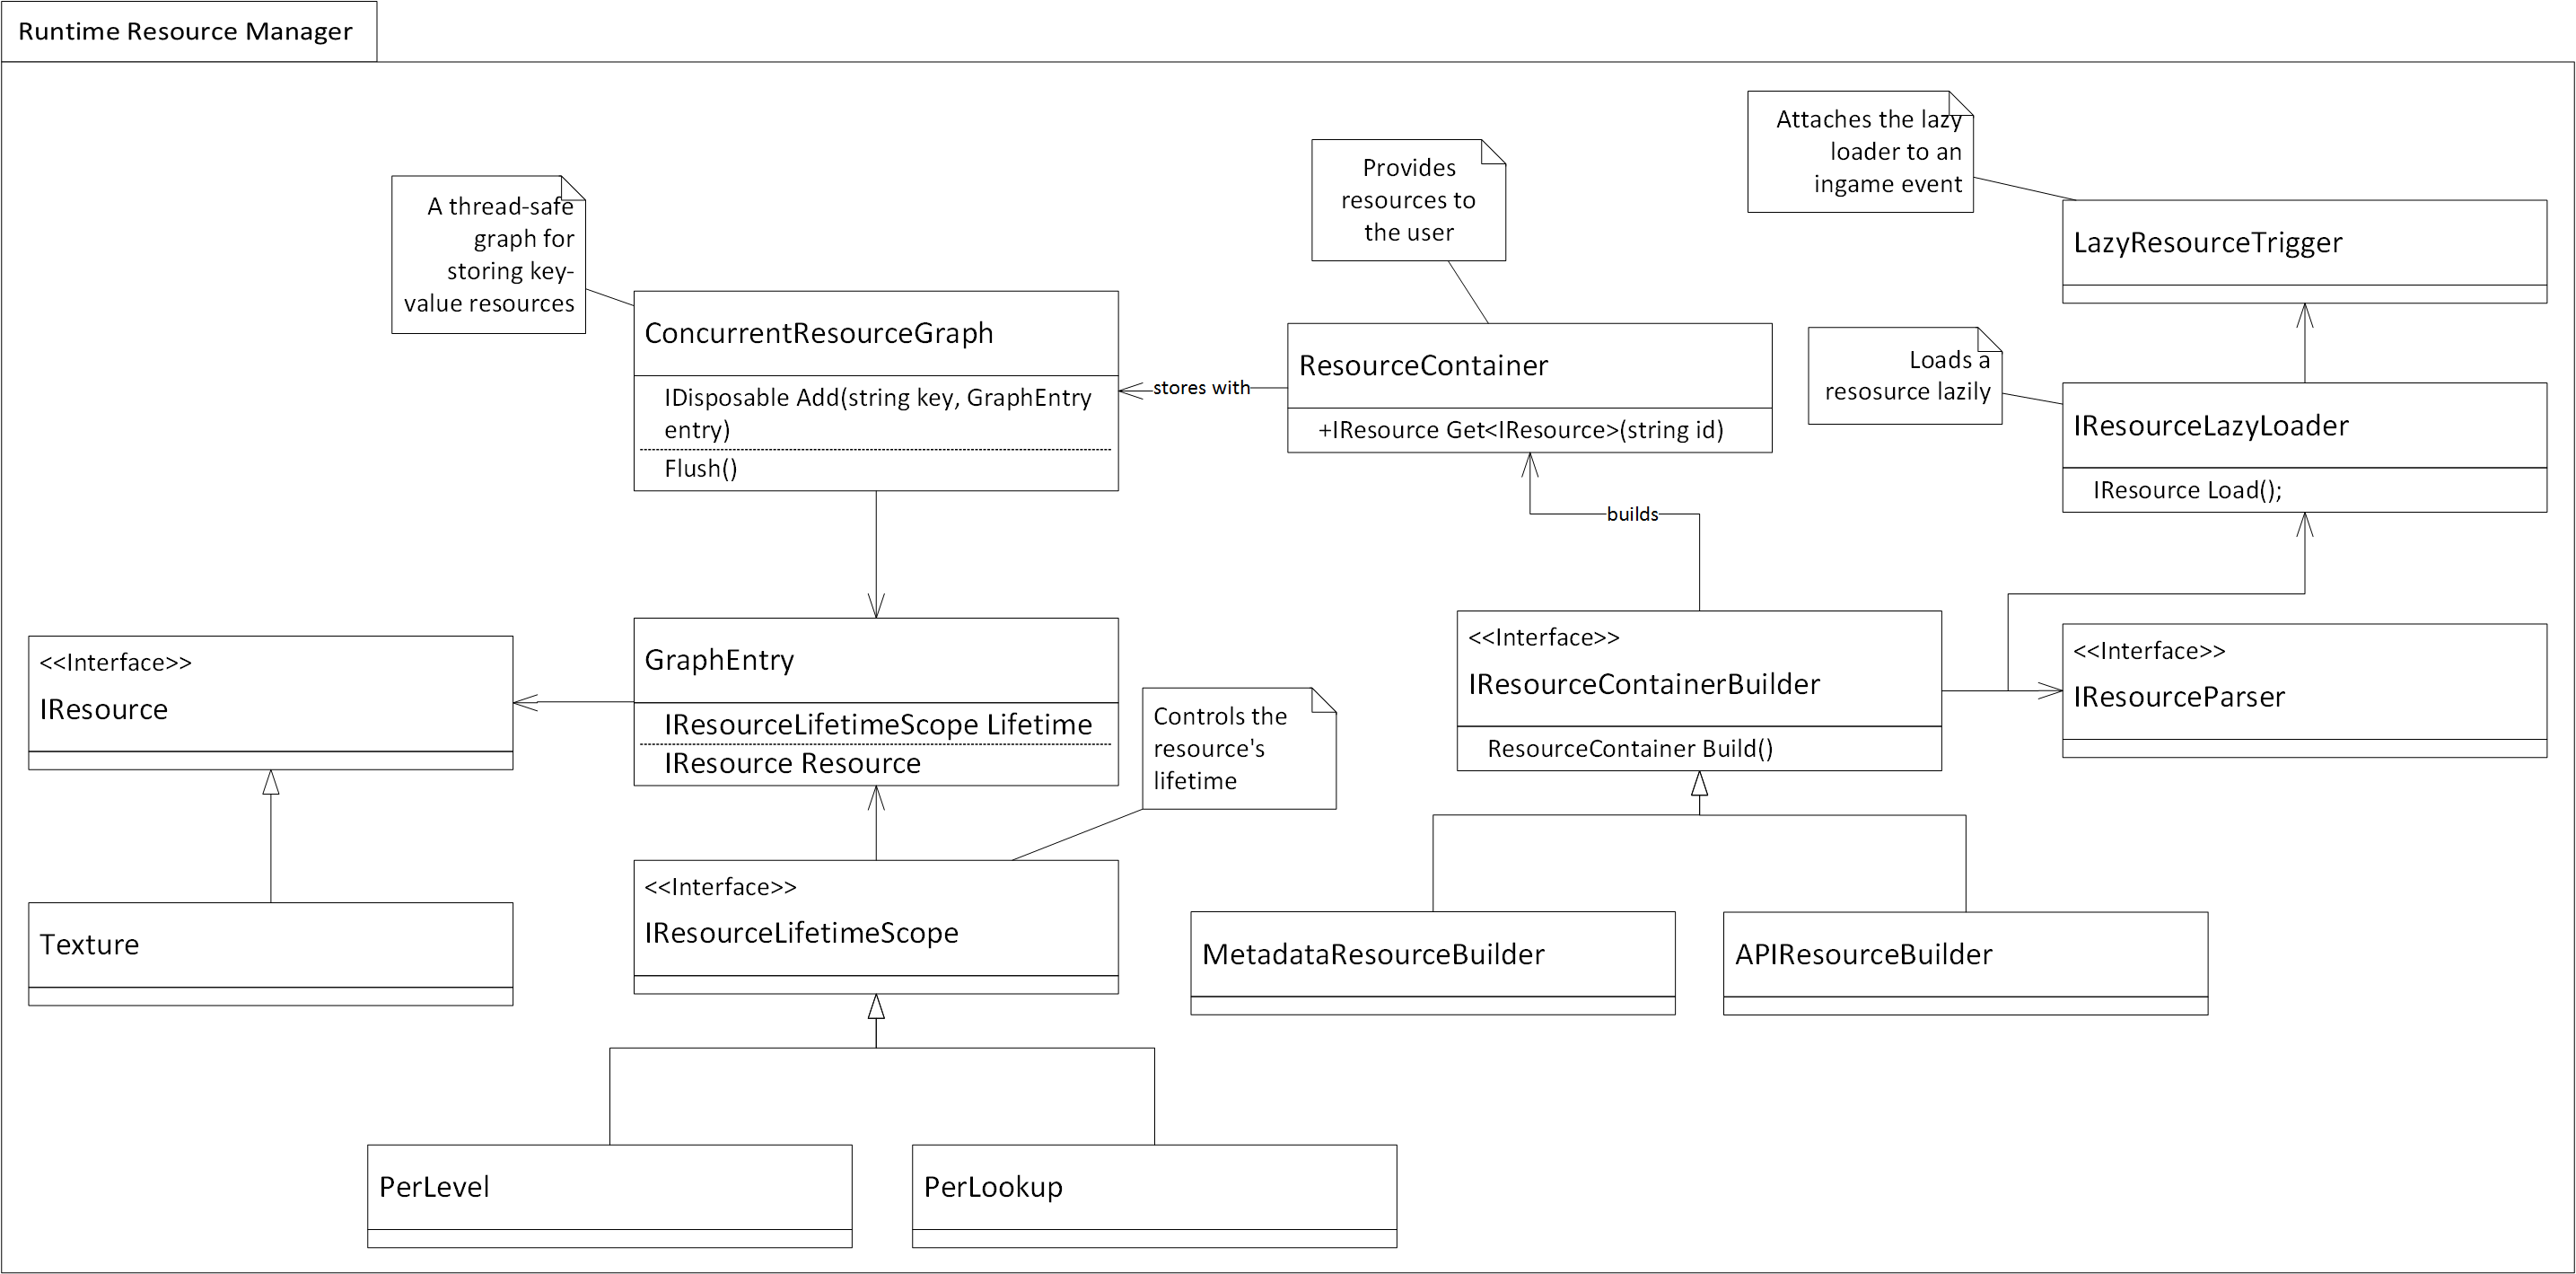
\includegraphics[width=165mm]{Images/runtime_resource_manager}
	\caption{UML του διαχειριστή πόρων πραγματικού χρόνου}
	\label{fig:runtime_resource_uml}
\end{figure}

\section{Τεχνητή νοημοσύνη}
Η τεχνητή νοημοσύνη χρησιμοποιείται για να παράγει ευφυείς συμπεριφορές κυρίως χαρακτήρες εκτός του παίχτη (NPCS). Οι αλγόριθμοι της τεχνικής νοημοσύνης προσπαθούν να προσομοιώσουν την ανθρώπινη συμπεριφορά και βασίζονται σε τεχνικές από θεωρία ελέγχου, ρομποτική και γενικά της πληροφορικής. Στα ηλεκτρονικά παιχνίδια η νοημοσύνη συμβάλει στο πιο ρεαλιστικό gameplay μέσα στους περιορισμούς του περιβάλλοντος. Η προσέγγιση είναι εντελώς διαφορετική από την τεχνητή νοημοσύνη σε άλλα πεδία, γιατί οι ικανότητες του υπολογιστή πρέπει να είναι ήπιες ώστε να δώσει σε ανθρώπινους παίκτες μια αίσθηση δικαιοσύνης και ικανοποίησης \cite{Sousa:2002:GPO:580160}.
 
\subsection{Δέντρα συμπεριφoρών}	
To δέντρο συμπεριφορών (behavior tree) είναι ένα δέντρο με ιεραρχικά συνδεδεμένους κόμβους για έλεγχο της ροής της διαδικασίας λήψης αποφάσεων μιας οντότητας με νοημοσύνη. Στα φύλλα του δέντρου βρίσκονται οι εντολές και η συμπεριφορά της οντότητας. Τα κλαδιά τα δημιουργούν διάφοροι τύποι κόμβων οι οποίοι περιέχουν εντολές και περιορισμούς για τη διάβαση του δέντρου \cite{champandard2007understanding}.

Η βασική οντότητα του δέντρου είναι ο κόμβος. Ο κάθε κόμβος αξιολογείται σε κάθε βήμα διάβασης του δέντρου και επιστρέφει την κατάστασή του:
\begin{description}
	\item [Success] Ο κόμβος αξιολογήθηκε με επιτυχία
	\item [Failure] Ο κόμβος αξιολογήθηκε με αποτυχία
	\item [Running] Ακόμη να τελειώσει η αξιολόγηση του κόμβου.
\end{description}

Η διάβαση του δέντρου προχωράει ανάλογα με την κατάσταση του προηγούμενου κόμβου. Οι κόμβοι αξιολόγησης λειτουργούν σαν λογικές πύλες.

\begin{description}
	\item [Sequence] Προσομοιώνει την πύλη AND, για να αξιολογηθεί ο κόμβος κλαδί με επιτυχία, πρέπει όλοι οι κόμβοι του κλαδιού να αξιολογηθούν επιτυχώς.
	\item [Selector] Προσομοιώνει την πύλη ΟR. Η αξιολόγηση του κλαδιού θεωρείται επιτυχημένη στην πρώτη αξιολόγηση ενός δέντρου με επιτυχία.
	\item [Random Selector] Ίδια συμπεριφορά με τον selector, απλά η αξιολόγηση των κόμβων γίνεται με τυχαία σειρά.
	\item [Random Sequence] Ίδια συμπεριφορά με το sequence, απλά η αξιολόγηση των κόμβων γίνεται με τυχαία σειρά.
\end{description}
	
H συμπεριφορά και αξιολόγηση των κόμβων μπορεί να μεταβληθεί χρησιμοποιώντας το decorator pattern \cite{Gamma:1995:DPE:186897}.

\begin{description}
	\item [Inverter] Ο κόμβος ο οποίος είναι decorated από τον inverter, επιστρέφει το αντίστροφο αποτέλεσμα κατά την αξιολόγηση.
	\item [Repeat Until Success] O κόμβος αξιολογείται ως Running εφόσον αξιολογηθεί με αποτυχία. 
	\item [Repeater] Η αξιολόγηση του κόμβου επαναλαμβάνεται ανάλογα με το προκαθορισμένο αριθμό επαναλήψεων
	\item [Max Time] Η αξιολόγηση γίνεται μέσα σε στα πλαίσια χρονικού διαστήματος.
\end{description}

Τα φύλλα του δέντρου καθορίζουν την πραγματική συμπεριφορά της νοημοσύνης. Τα φύλλα μπορούν να είναι:

\begin{description}
	\item [Ερωτήσεις] Για παράδειγμα: υπάρχει το συγκεκριμένο αντικείμενο στο χάρτη;
	\item [Συμπεριφορά] Για παράδειγμα: προχώρα ένα βήμα μπροστά.
\end{description}

Στο mind map \ref{fig:behavior_trees_mind_map} παρουσιάζονται οι σχέσεις και οι τύποι των κόμβων.
\begin{figure}[h!]
	\centering
	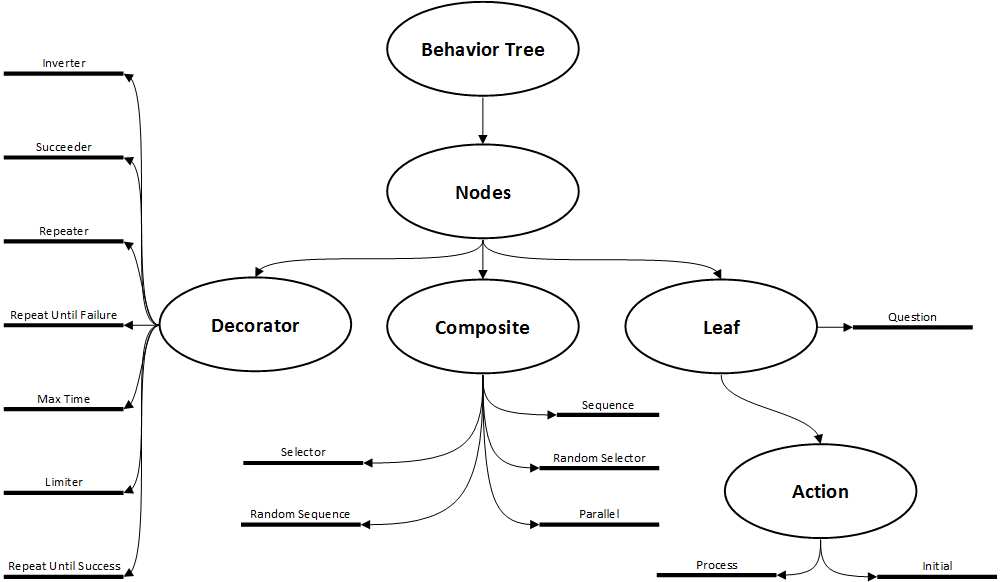
\includegraphics[width=165mm]{Images/behavior_trees}
	\caption{Δέντρο συμπεριφορών}
	\label{fig:behavior_trees_mind_map}
\end{figure}
	
\paragraph{API}
Στο \gls{API} του υποσυστήματος συμπεριλαμβάνεται ένα fluent tree builder για εύκολη δημιουργία δέντρων στη μνήμη με κώδικα και ένας οραματιστής δέντρου (tree visualizer) για απόδοση του δέντρου στην οθόνη με αξιολόγηση και ενημέρωση πραγματικού χρόνου για αποσφαλμάτωση. Στο παράδειγμα κώδικα \ref{fsm_builder} παρουσιάζεται η μοντελοποίηση της συμπεριφοράς ενός χαρακτήρα ο οποίος προσπαθεί να βρει την έξοδο σε ένα λαβύρινθο με εχθρούς.

	\lstset
	{
		style=sharpc, 
		caption={Behavior tree builder}		
	}
	\begin{lstlisting}[label=fsm_builder]
 behaviorBuilder
 .Selector(name: "Move to end")
	 .Decorate(For.RepeatUntilFailure)
		 .Sequence(name: "try walk")
			 .Question(CheckNextTile, name: "next tile empty?")
			 .Behavior(MoveOneTile, name: "go 1 step forward")
	 .Sequence("key obstacle")
			 .Question(CheckTileForKey, name: "found key?")
			 .Selector("handle key")
	 .End
	 .Sequence
	 .DecorateFor(Decorator.AlwaysSuccess)
		 .Behavior(RunAway)
	 .End
 .End
 .Tree;
	\end{lstlisting}


\subsection{Finite State Machines}	
 Finite state machine είναι μια αφηρημένη μηχανή η οποία μπορεί να βρίσκεται σε μία από ένα πεπερασμένο αριθμό καταστάσεων και με την επέλευση κάποιου γεγονότος μπορεί να αλλάξει από μια κατάσταση σε άλλη. 
 Κατάσταση (state) είναι η περιγραφή της κατάστασης στην οποία βρίσκεται το σύστημα \cite{gill1962introduction}.
 Γεγονός (event) δράση η οποία οδηγεί σε αλλαγή κατάστασης.
 Transition (μετάβαση) είναι ένα σύνολο δράσεων που πρέπει να εκτελεστούν όταν πληρείται μια προϋπόθεση ή όταν συμβεί ένα γεγονός. Στο \gls{UML} \ref{fig:state_machine_uml} παρουσιάζονται οι σχέσεις μεταξύ των οντοτήτων του finite state machine.
 
\begin{figure}[h!]
	\centering
	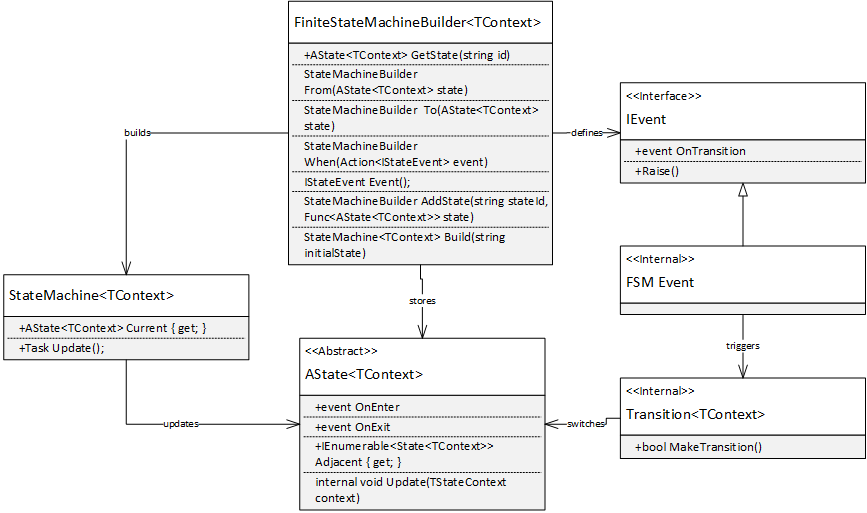
\includegraphics[width=165mm]{Images/state_machine_uml}
	\caption{UML του υποσυστήματος των state machines }
	\label{fig:state_machine_uml}
\end{figure}	

Στο παράδειγμα \ref{fig:state_machine_example} μοντελοποιούνται οι καταστάσεις και τα γεγονότα τα οποία οδηγούν σε αλλαγή κατάστασης ενός χαρακτήρα με νοημοσύνη. Ο χαρακτήρας αυτός περιπλανιέται τυχαία, όταν συναντήσει αντικείμενο το μαζεύει και όταν συναντήσει εχθρό τον πολεμά. Αν ο εχθρός είναι πιο δυνατός, τότε αποφεύγει την μάχη φεύγοντας.
\begin{figure}[h!]
	\centering
	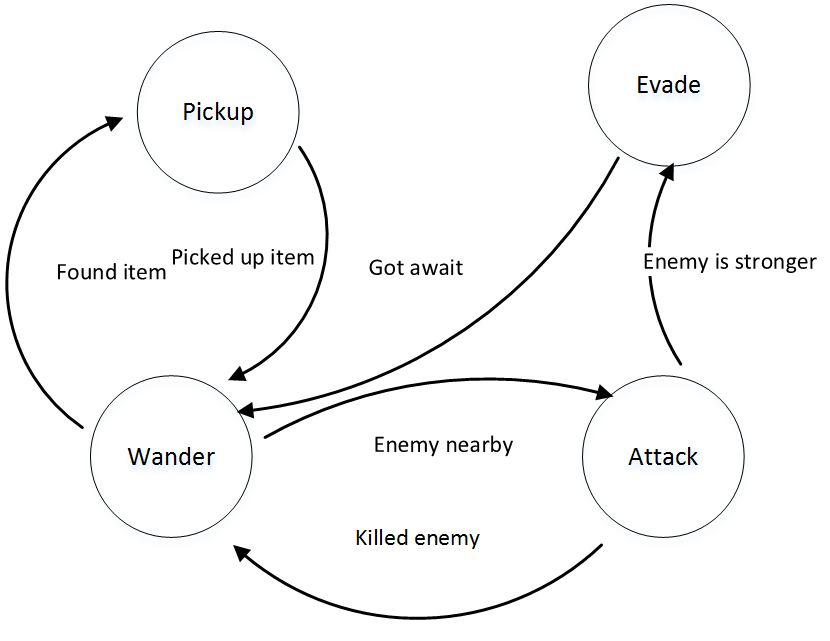
\includegraphics[width=100mm]{Images/ingame_fsm_example}
	\caption{Παράδειγμα state machine}
	\label{fig:state_machine_example}
\end{figure}

H σύνδεση του finite state machine γίνεται μέσω του builder \cite{Gamma:1995:DPE:186897}. Στον builder γίνεται καταχώρηση τον καταστάσεων μέσω μιας μεθόδου-factory και δημιουργία αυτοενεργοποιημένων συμβάντων ή συμβάντων τα οποία ενεργοποιούνται από τον χρήστη τα οποία οδηγούν σε αλλαγή κατάστασης. Μετά γίνεται το κτίσιμο του FSM και η ενημέρωση του με βάση το γενικότερο πλαίσιο. Παράδειγμα χρήσης του builder παρουσιάζεται στο παράδειγμα κώδικα \ref{lst:fsm_builder}.

\lstset
{
	style=sharpc, 
	caption={State machine API}
}
\begin{lstlisting}[label=lst:fsm_builder]
fsmBuilder
.AddState("PickUp",() => new PickupState())
.AddState("Wander",() => new WanderState())
//with lifetime
.AddState("Attack",() => ioc.Resolve<AttackState>())
.AddState("Evade",() => new EvadeState())	
		
var attackEvent = fsmBuilder
.From("Wander")
.To("Pickup")
.When(context=> context.FoundItem) //auto triggered
	
var attackEvent = fsmBuilder
.From("Wander")
.To("Attack")
.Event() //manually triggered
	 	
world.OnCollision += (sender,args)=>
{
    if(args.CollidedType is Enemy)
	    attackEvent.Trigger();
}
	 
//emitted	 
var playerBehaviorFsm = fsmBuilder.Build("Active);
await playerBehaviorFsm.Update(playerContext);
	
\end{lstlisting}
